\documentclass{beamer}
\usepackage{amsfonts,amsmath,oldgerm}
\usetheme{sintef}
\usepackage{xeCJK}
\usepackage[absolute,overlay]{textpos}
\newcommand{\testcolor}[1]{\colorbox{#1}{\textcolor{#1}{test}}~\texttt{#1}}

\usefonttheme[onlymath]{serif}

\titlebackground*{assets/sdubackground}

\newcommand{\hrefcol}[2]{\textcolor{cyan}{\href{#1}{#2}}}

\title{独家!直击计算机系高年级生,竟集体“窝藏”神秘笔记!}
\subtitle{知情学长不忍了:四年规划秘籍,今天一次全公开!}
% \course{Master's Degree in Computer Science}
\author{22软件三杨熙承}
% \IDnumber{1234567}
\date{2025/9}

\begin{document}
\maketitle

% \begin{frame}

% This template is a based on \hrefcol{https://www.overleaf.com/latex/templates/sintef-presentation/jhbhdffczpnx}{SINTEF Presentation} from \hrefcol{mailto:federico.zenith@sintef.no}{Federico Zenith} and its derivation \hrefcol{https://github.com/TOB-KNPOB/Beamer-LaTeX-Themes}{Beamer-LaTeX-Themes} from Liu Qilong

% \vspace{\baselineskip}

% THU style adaptation contributed by \hrefcol{https://github.com/FangWHao}{Wenhao Fang}

% SDU style adaptation contributed by \hrefcol{https://github.com/almostgph}{Penghong Gao}


% \vspace{\baselineskip}

% In the following you find a brief introduction on how to use \LaTeX\ and the beamer package to prepare slides, based on the one written by \hrefcol{mailto:federico.zenith@sintef.no}{Federico Zenith} for \hrefcol{https://www.overleaf.com/latex/templates/sintef-presentation/jhbhdffczpnx}{SINTEF Presentation}

% \vspace{\baselineskip}

% This template is released under \hrefcol{https://creativecommons.org/licenses/by-nc/4.0/legalcode}{Creative Commons CC BY 4.0} license

% \end{frame}

%================================================================
% 知乎声音引入部分
%================================================================
\section*{开篇之前:一些来自网络的声音}

\begin{frame}{网络热门回答(一)}
    \begin{block}{学霸和“学渣”}
    “我大学最好的朋友,一个拿了国奖的学霸,绩点专业第一。毕业后去面试,发现自己会的企业都用不上,\textbf{企业要的他都不会}。他甚至不知道什么是 Docker,没用 Git 做过项目协同。反倒是我这种天天逃课在宿舍自己搞项目的‘学渣’,因为实习早,早早拿到了offer。”
    \end{block}
    \begin{block}{我这两年到底学了些什么?}
    “我按部就班地听课、完成作业,绩点也还行。但前几天我试着去投了一下暑期实习,简历关都过不了。我看了看那些招聘要求,什么Spring Boot、Vue、Redis、分布式、微服务……我一个都没在课上听过。我开始严重怀疑,我这两年到底学了些什么?感觉自己像个傻子,和那些高中毕业就开始在培训班学习的同学比,好像没什么优势。”
    \end{block}
\end{frame}

\begin{frame}{网络热门回答 (二)}
    \begin{block}{学校领进门,修行靠个人}
    “说实话,我的编程能力、算法能力,基本上都是靠B站上的各种教程、国外的CS61A、CSAPP这些神级公开课,还有刷LeetCode练出来的。学校的课程帮我构建了一个知识索引,让我知道‘哦,原来还有个东西叫操作系统’,‘还有个东西叫计算机网络’,但具体这些东西是怎么回事,怎么在实际中运用,都得靠自己去网上找资源学。”
    \end{block}
    \begin{block}{90\%的学习发生在那块屏幕上}
    “回过头看,大学四年对我最大的作用,就是给了我一个学生身份,让我有时间和机会去自学。它提供了一个环境,但知识和技能的获取,90\%都发生在那块小小的屏幕和键盘上,而不是教室里。”
    \end{block}
\end{frame}

\begin{frame}{那么,这些声音告诉了我们什么?}
\begin{itemize}
    \item 我们从小被告知,学习是一场关于成绩、排名的比拼。
    \item 我们拼尽全力,成为老师眼中的好学生,父母口中的骄傲,我们以为自己赢了...
    \item 也许高中确实如此。
    \item \alert{但,大学这真的是唯一的赛道吗?}
    \item 在这座象牙塔之外,存在着一个截然不同的真实世界。那个世界里,企业在招聘,技术在迭代,需求在变化,如今的就业形式也并不乐观。
    \item 可悲的是,\alert{那里的游戏规则,我们甚至一无所知。}
\end{itemize}
\end{frame}

\section*{怎么做?}

\begin{frame}{我们的目标:一份「双赢」的四年规划}
    \begin{center}
        \Large
        成年人不做选择,\alert{我们全都要!}
    \end{center}


    \begin{columns}[T]
        \begin{column}{0.5\textwidth}
            \Large\textbf{玩转「校内赛道」}
            \vspace{0.2cm}
            \begin{itemize}
                \item 追求成绩,但绝非盲目刷分。
                \item 我们要的是\alert{“有效成绩”}:精准投入,高效学习,深刻理解核心课程。
                \item 拒绝“无效内卷”,把时间花在刀刃上。
            \end{itemize}
        \end{column}
        
        \begin{column}{0.5\textwidth}
            \Large\textbf{开拓「校外战场」}
            \vspace{0.2cm}
            \begin{itemize}
                \item 同步构建面向未来的“实战技能树”。
                \item 我们要的是\alert{“硬核能力”}:紧跟业界技术,上手真实项目,积累宝贵经验。
                \item 拒绝“闭门造车”,让能力与市场接轨。
            \end{itemize}
        \end{column}
    \end{columns}

    % \uncover<2->{
    % \vspace{0.5cm}
    % \rule{\textwidth}{0.4pt}
    % \vspace{0.3cm}
    % \begin{center}
    %     \textbf{核心思想:这两条路并非二选一,而是相辅相成、必须并行。} \\
    %     接下来的分享,我将为大家详细拆解,在大学的每一年,我们具体应该做什么。
    % \end{center}
    % }
\end{frame}


\section{第0步}

\begin{frame}{一份CS自学宝典}
    \framesubtitle{CS DIY Wiki --- \hrefcol{https://csdiy.wiki/}{https://csdiy.wiki/}}

    \begin{columns}[T]
        \begin{column}{0.45\textwidth}
            \begin{figure}
                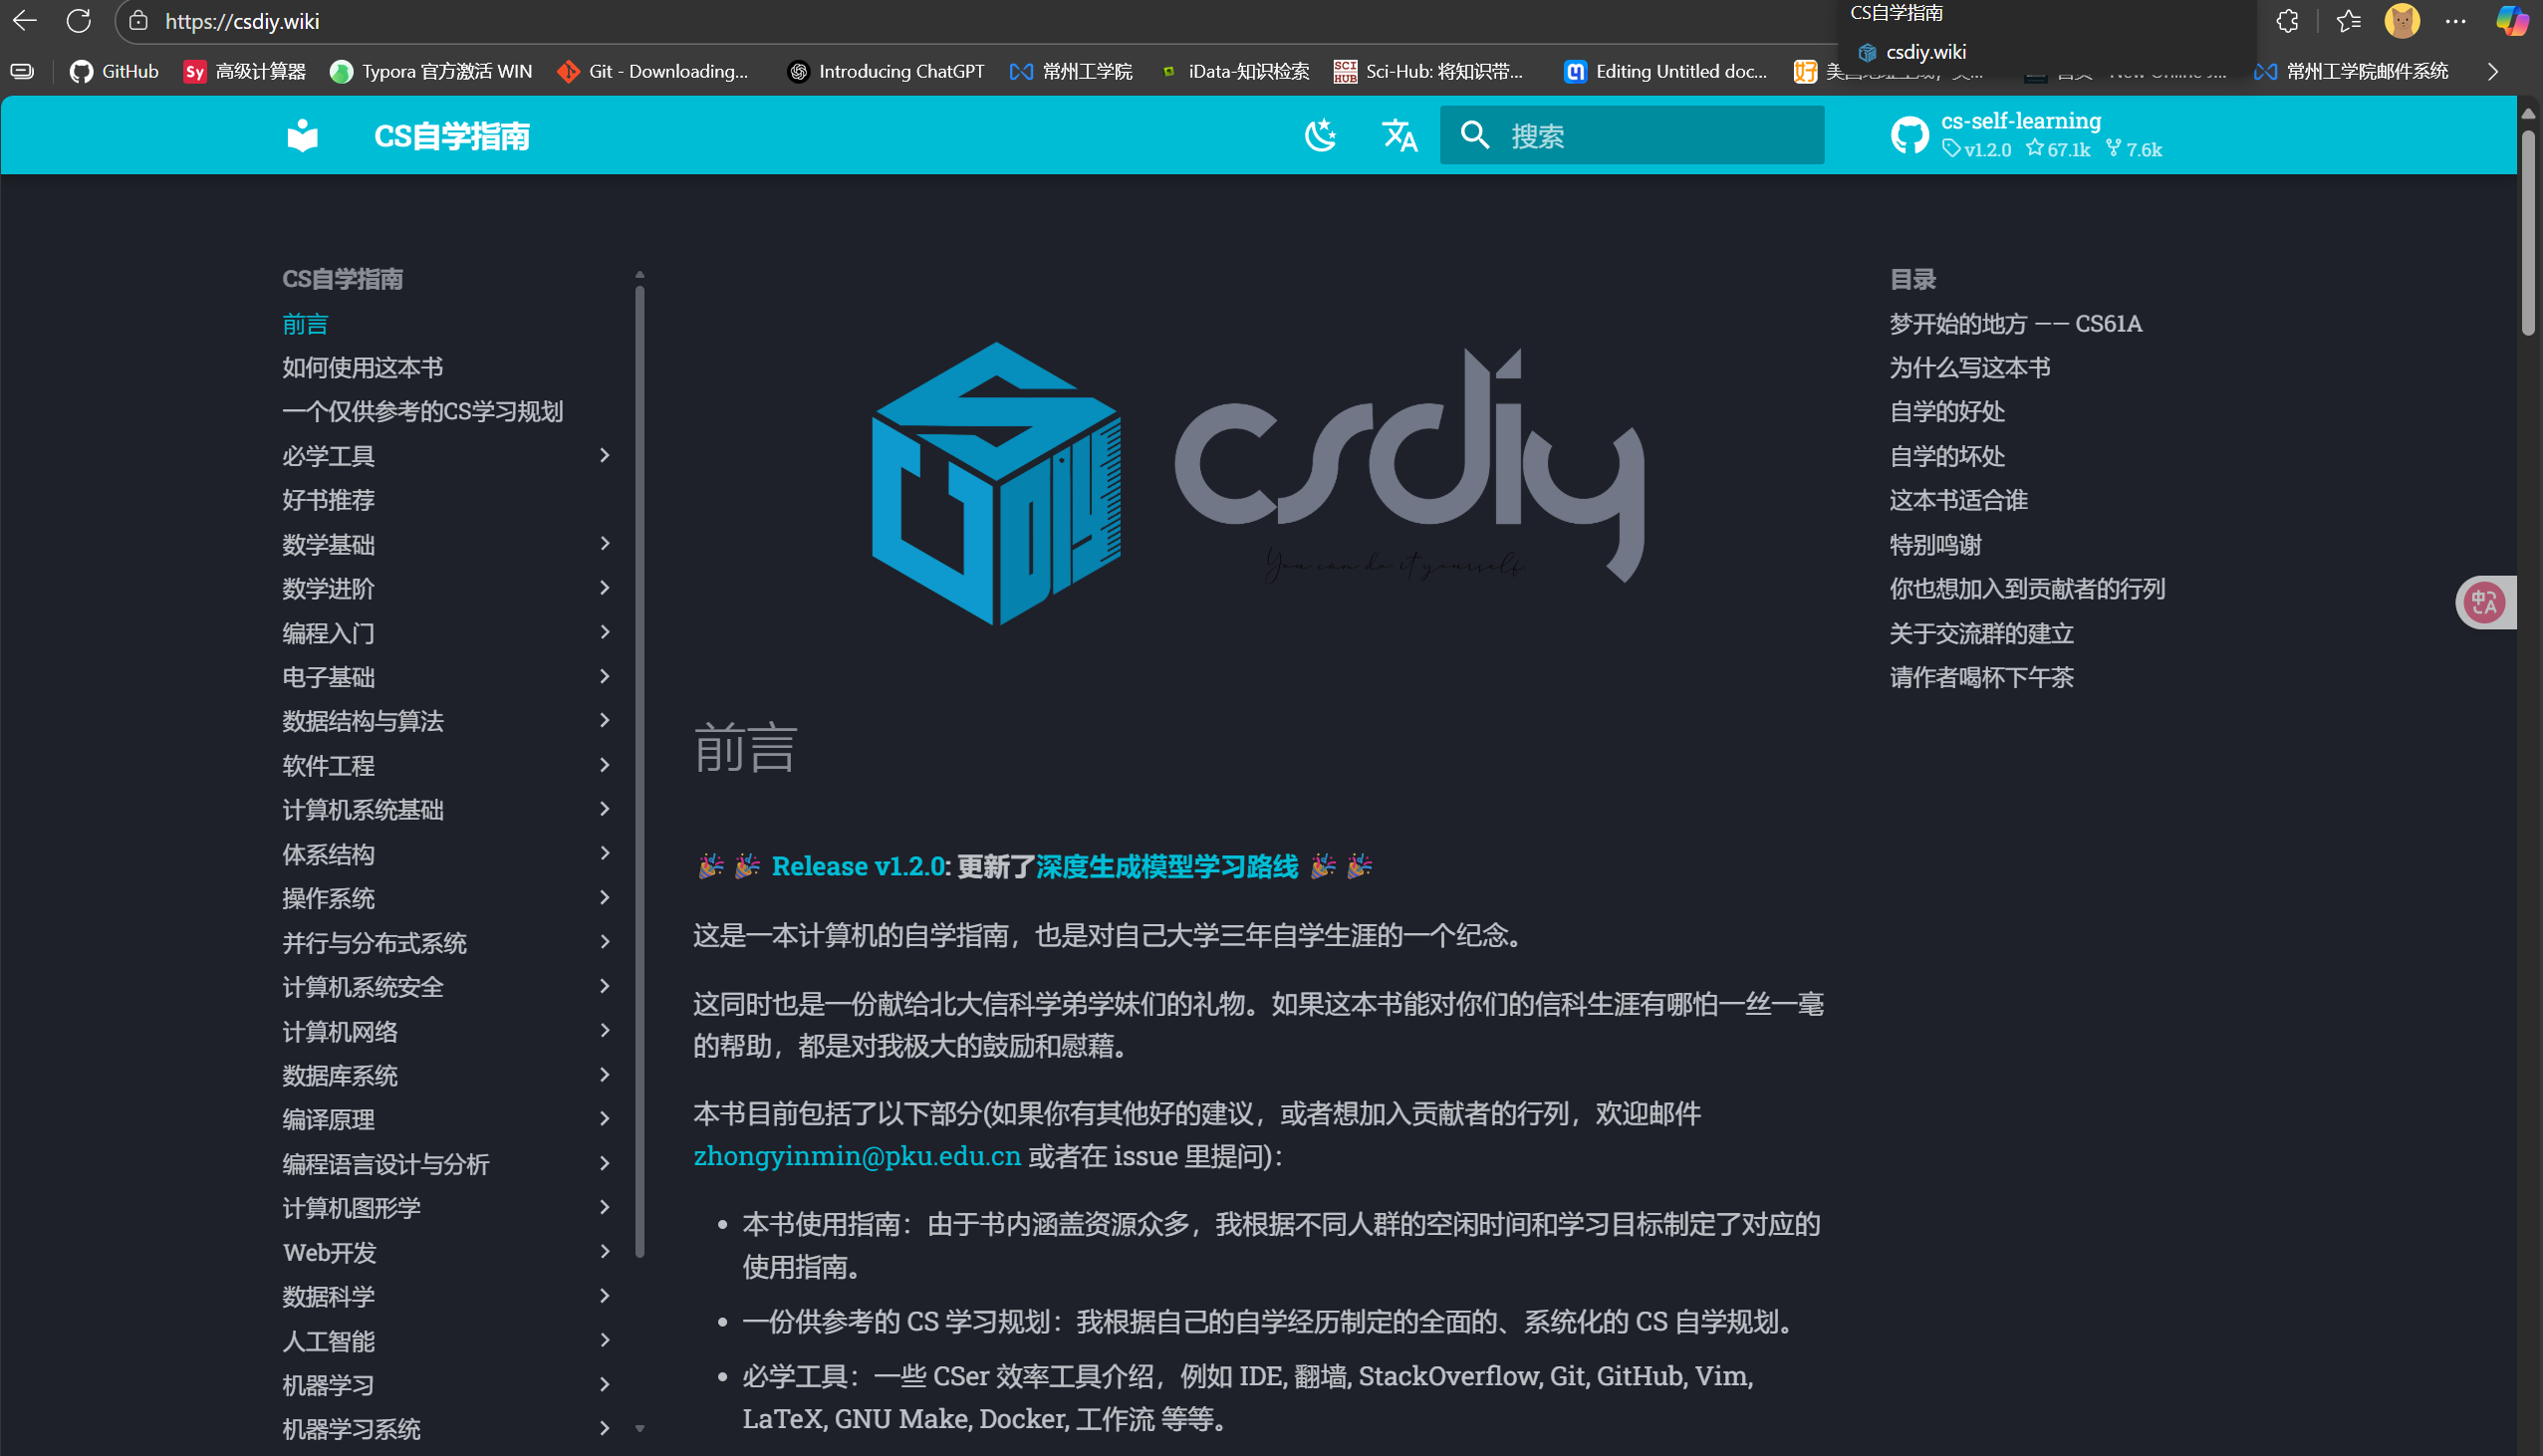
\includegraphics[width=\textwidth]{assets/cs.png}
                % \caption{}
            \end{figure}
        \end{column}

        \begin{column}{0.55\textwidth}
            \Large \textbf{这是什么?}
            \begin{itemize}
                \item 一个由北大学长维护的CS学习资源库网站。
                \item 它为你规划了从大一到大四的知识体系,并整理了全世界\alert{最优质}的免费公开课。
                \item 你的很多困惑,这里都有答案。
            \end{itemize}
        \end{column}
    \end{columns}

\begin{flushright}
    \small\textit{* P.S. 本人也是该开源项目的贡献者之一哦!}
\end{flushright}
    
\end{frame}

\begin{frame}{拉开差距的第一步}
    \begin{center}
        \Large
        开学时,大家的智商、分数其实都在一条水平线上。
        \vspace{0.5cm}

        但一年之后,有的人似乎“开了窍”,有的人却还在原地踏步。
    \end{center}
    \vfill

    \begin{alertblock}{你有没有想过,真正的分水岭是什么?}
        最关键的,不是你比别人多熬了几个夜,也不是你比别人多刷了几道题...
        \vspace{0.5cm}
        \begin{center}
            \Huge\alert{是你使用「工具」的效率和认知!}
        \end{center}
    \end{alertblock}

\end{frame}

\begin{frame}{你的第一个超级工具:AI}
    \begin{columns}[T]
        \begin{column}{0.5\textwidth}
            \Large\textbf{AI 能帮你做什么?}
            \begin{itemize}
                \item \textbf{快速解释概念} \\
                \small 看不懂的知识点?直接问它,让它用各种比喻给你讲明白。
                \item \textbf{代码纠错优化} \\
                \small 帮你找Bug,解释报错,甚至给你重构代码的建议。
                \item \textbf{开拓编程思路} \\
                \small 写项目没头绪?让它给你提供几种不同的实现方案。
            \end{itemize}
        \end{column}
        
        \begin{column}{0.5\textwidth}
            \Large\textbf{你应该如何利用AI?}
            \vspace{0.3cm}

            \uncover{
            \textit{把 AI 当成你的\alert{「领航员」},而不是\alert{「代驾」}。}
            % \vspace{0.cm}
            }
            
            \begin{alertblock}{绝对禁止!!!}

            \textbf{不假思索的直接复制粘贴} AI 生成的代码去完成必要的任务!这是\alert{学术不端}行为,同时让你失去了学习的机会!

            \end{alertblock}

        \end{column}
    \end{columns}
\end{frame}

\begin{frame}{四大主流AI模型}
    \begin{columns}[T]
        \begin{column}{0.5\textwidth}
            % --- GPT ---
            \begin{center}
                
\includegraphics[height=2cm]{assets/openai.png} \\
                \large\textbf{GPT (OpenAI)}
            \end{center}
            \begin{itemize}
                \item 堪称AI模型中的“瑞士军刀”,功能多样,能满足多种需求。
                \item 搜索信息能力断档式领先
                \item 祖师爷
            \end{itemize}
        \end{column}

        \begin{column}{0.5\textwidth}
            % --- Claude ---
            \begin{center}
                
\includegraphics[height=2cm]{assets/claude.png} \\
                \large\textbf{Claude (Anthropic)}
            \end{center}
            \begin{itemize}
                \item  擅长根据用户提供的写作范例,快速学习并适应其风格。
                \item  “公认最佳编程AI”,在AI编程平台中,像Bolt和Cursor等平台就将Claude4 Sonnet作为默认模型。
            \end{itemize}
        \end{column}
    \end{columns}
\end{frame}

\begin{frame}{四大主流AI模型}
    \begin{columns}[T]
        \begin{column}{0.5\textwidth}
            % --- Gemini ---
            \begin{center}
                
\includegraphics[height=2cm]{assets/gemini-ai.png} \\
                \large\textbf{Gemini (Google)}
            \end{center}
            \begin{itemize}
                \item 碾压式的视频处理能力,图像生成也不错
                \item 200万词的上下文窗口,这使其能够处理整本书、多个文档
                \item 回复精准精确。
            \end{itemize}
        \end{column}
        
        \begin{column}{0.5\textwidth}
            % --- Grok ---
            \begin{center}
                
\includegraphics[height=2cm]{assets/Grok.png} \\
                \large\textbf{Grok (xAI)}
            \end{center}
            \begin{itemize}
                \item 回答风格更具个性和幽默感,不回避争议性话题。
                \item 实时信息更新功能
            \end{itemize}
        \end{column}
    \end{columns}
\end{frame}

\begin{frame}
    % 背景图片:梯子靠在高墙上
    \begin{textblock*}{\textwidth}(0.35\paperwidth, 0.1\paperheight)
        
\includegraphics[height=0.8\paperheight]{assets/梯子.png}
    \end{textblock*}

    % ================================================================
    %   文字像思绪一样,散落在梯子和墙的周围
    % ================================================================

    \begin{textblock*}{6cm}(0.25\paperwidth, 0.1\paperheight)
        \Large 梯子,
        \normalsize 能带你看到...
    \end{textblock*}

    \begin{textblock*}{7cm}(0.65\paperwidth, 0.2\paperheight)
        \huge 一片新天地
    \end{textblock*}

    \begin{textblock*}{5cm}(0.3\paperwidth, 0.5\paperheight)
        \large 但请记住...
    \end{textblock*}

    \begin{textblock*}{6.5cm}(0.7\paperwidth, 0.55\paperheight)
        \Large 爬得越高,风越大
    \end{textblock*}
    
    \begin{textblock*}{5cm}(0.75\paperwidth, 0.65\paperheight)
        \small ...脚要踩稳
    \end{textblock*}

    \begin{textblock*}{12cm}(0.05\paperwidth, 0.8\paperheight)
        \large 最重要的是,我们的目的是为了,
    \end{textblock*}
    \begin{textblock*}{12cm}(0.72\paperwidth, 0.8\paperheight)
        \large \textbf{欣赏和学习外面的风景},
    \end{textblock*}
    \begin{textblock*}{12cm}(0.3\paperwidth, 0.9\paperheight)
        \large 而不是为了 \alert{翻进别人的院子}。
    \end{textblock*}

\end{frame}
% {https://aistudio.google.com/prompts/new_chat}

\begin{frame}{第二张「身份证」:Git \& GitHub}
    \begin{columns}[T]
        \begin{column}{0.5\textwidth}
            \begin{figure}
                
\includegraphics[width=0.7\textwidth]{assets/github.png}
                \caption{面试官百分之百会点开的链接}
            \end{figure}
        \end{column}
        
        \begin{column}{0.5\textwidth}
            \Large
            对于程序员来说,\\
            GitHub Profile 就是...
            \vfill

            \begin{itemize}
                \item \huge 你的代码时光机
                \vfill
                \item \huge 你的作品展览馆
                \vfill
                \item \huge \alert{你的技术新简历}
                \vfill
                \item \huge 你的成长路线图
            \end{itemize}
        \end{column}
    \end{columns}

\end{frame}

\begin{frame}{写作的「轻」与「重」:Markdown \& LaTeX}
    \framesubtitle{让内容与格式分离,专注于思考本身}

    \begin{columns}[T]
        \begin{column}{0.5\textwidth}
            \begin{center}
                \Large\textbf{Markdown:简洁的艺术}
                \vspace{0.2cm}
                \\
                \large \textit{你的写作「T恤衫与牛仔裤」}
            \end{center}
            
            \begin{itemize}
                \item \textbf{用在哪?} \\
                \small 快速记录笔记、撰写项目文档(\texttt{README.md})、发技术博客...
                \item \textbf{什么感觉?} \\
                \small \alert{五分钟上手,轻便高效。} 语法简单,让你完全专注于内容。
            \end{itemize}
        \end{column}

        \begin{column}{0.5\textwidth}
            \begin{center}
                \Large\textbf{LaTeX:专业的极致}
                \vspace{0.2cm}
                \\
                \large \textit{你的学术「西装与燕尾服」}
            \end{center}
            
            \begin{itemize}
                \item \textbf{用在哪?} \\
                \small 撰写学术论文、排版复杂数学公式 ...\\
                $
        \langle \Omega | T \{ \phi(x_1) \dots \phi(x_n) \} | \Omega \rangle = \frac{\int \mathcal{D}\phi \, \phi(x_1) \dots \phi(x_n) \exp \left( i S[\phi] \right)}{\int \mathcal{D}\phi \, \exp \left( i S[\phi] \right)}
                $
                \item \textbf{什么感觉?} \\
                \small \alert{排版界的“降维打击”。} 追求极致的专业与美感。
                \item \footnotesize \textit{(P.S. 本次讲座的PPT就是用LaTeX制作的)}
            \end{itemize}
        \end{column}
    \end{columns}

\end{frame}

\begin{frame}{像专家一样使用搜索引擎}
    \begin{columns}[T]
        \begin{column}{0.4\textwidth}

            \begin{alertblock}{Google}
                全球信息质量的顶尖选择,尤其在英文技术资料方面无出其右。
            \end{alertblock}

            \begin{alertblock}{Bing (国际版)}
                整合了强大的AI(Copilot),能够提供更智能的总结和答案,访问也更便捷。
            \end{alertblock}

            
        \end{column}
        
        \begin{column}{0.6\textwidth}
            \Large\textbf{必须掌握的检索规范}
            \begin{itemize}
                \item \textbf{精准匹配 (\texttt{"..."})}
                    \begin{itemize}
                    \item \small  搜索 \texttt{"常州工学院"},将只匹配完整包含“常州工学院”的页面
                    \end{itemize}
                
                \item \textbf{不包含关键字 (\texttt{-})}

                \item \textbf{包含关键字 (\texttt{+})}
  
                \item \textbf{搜索特定文件类型 (\texttt{filetype:})}
                    \begin{itemize}
                    \item \small  \texttt{计算机组成原理 filetype:pdf}
                    \end{itemize}

                \item \textbf{搜索特定网址 (\texttt{site:})}
                    \begin{itemize}
                    \item \small  \texttt{data structure site:stackoverflow.com}
                    \end{itemize}
            \end{itemize}
        \end{column}
    \end{columns}
\end{frame}



\begin{frame}{Linux:从“图形界面”到“命令行”的飞跃}
    \begin{columns}[T]
        \begin{column}{0.5\textwidth}
            \begin{center}
                \Huge CLI > GUI
                \vspace{0.5cm}
                
                \Large \textbf{为什么要拥抱命令行?}
            \end{center}
            
            \begin{itemize}
                \item  你将从一个软件的“使用者”,变为一台计算机的\alert{“掌控者”}。
               
                \item  服务器、云计算、嵌入式、AI训练... 几乎所有严肃的开发环境,都构建于 \alert{Linux} 之上。
            \end{itemize}

        \end{column}
        
        \begin{column}{0.5\textwidth}
            \Large\textbf{新手入门路线图}
            \vspace{0.3cm}
            
            \begin{itemize}
                \item \textbf{安装 WSL} \\
                \small Windows Subsystem for Linux. 你在Windows上体验原生Linux的最佳方式(也是推荐的C语言开发环境)。
                
                \item \textbf{熟悉常用命令} \\
                \small 先玩转这几个:\texttt{ls, cd, mkdir, rm, mv, grep, ssh}
                
                \item \textbf{学习Shell脚本} \\
                \small 编写简单脚本,让重复性任务自动化,感受“偷懒”的极客乐趣。

                \item \textbf{必学课程} \\
                \small \hrefcol{https://missing.csail.mit.edu/2020/}{\textbf{“计算机教育中缺失的一课”}}
            \end{itemize}
        \end{column}
    \end{columns}

\end{frame}



\begin{frame}{浏览器插件}
\framesubtitle{沉浸式翻译、篡改猴.....}
    % --- 大图作为绝对的视觉主体 ---
    \begin{figure}
        \centering
        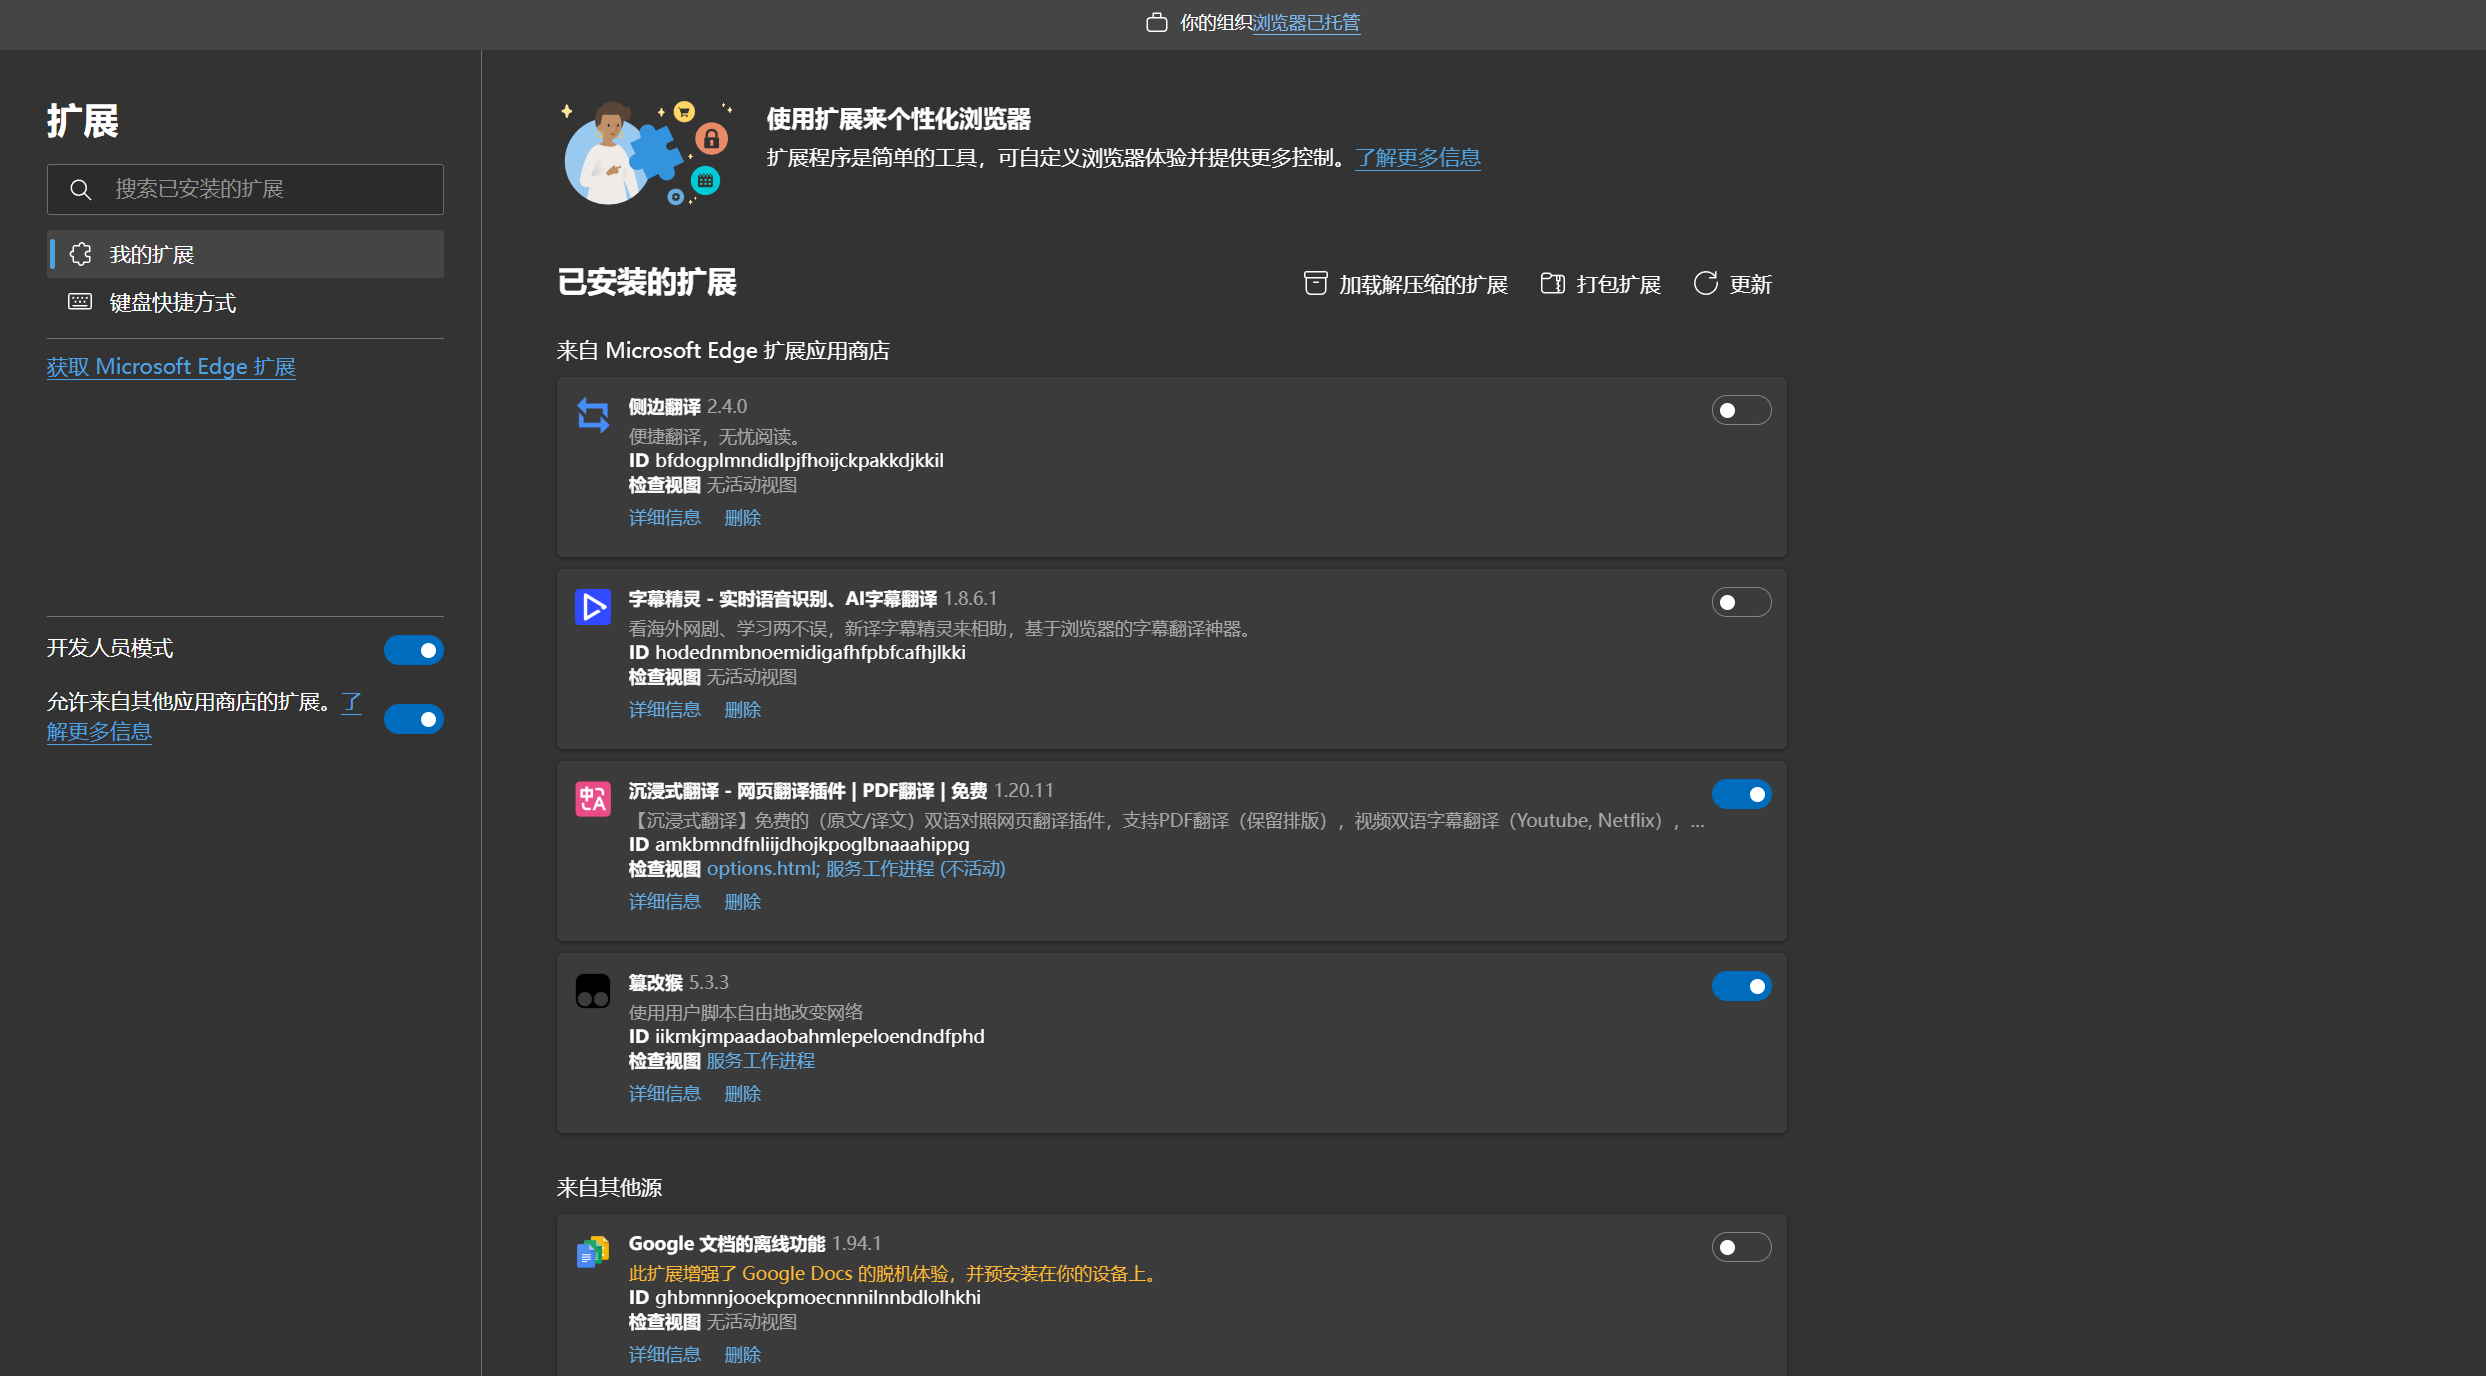
\includegraphics[width=0.85\textwidth]{assets/image.png}
    \end{figure}

\end{frame}


\begin{frame}{Docker \& K8s}
    \begin{columns}[T]
        \begin{column}{0.6\textwidth}
            % --- Docker ---
            \huge Docker
            \large\textit{软件的“集装箱”}
            \begin{itemize}
                \item  \textbf{解决什么问题?} \\
                \small 终结“在我电脑上明明能跑啊?”这个魔咒
                \item \textbf{它能做什么?} \\
                \small 在任何地方都能完美复现运行。
            \end{itemize}
            
            \vspace{0.5cm}
            
            % --- Kubernetes (K8s) ---
            \huge Kubernetes (K8s)
            \large\textit{集装箱的指挥官}
            \begin{itemize}
                \item  \textbf{解决什么问题?} \\
                \small 管理容器。现代云服务的基石。
            \end{itemize}
        \end{column}
        
        \begin{column}{0.4\textwidth}
            \begin{figure}
                \centering
                
\includegraphics[height=3cm]{assets/Docker.png}
            \end{figure}
            

            \begin{figure}
                \centering
                
\includegraphics[height=3cm]{assets/k8s.png}
            \end{figure}
        \end{column}
    \end{columns}
    \begin{textblock*}{8cm}(0.15\paperwidth, 0.92\paperheight) % 定位在右下角
        \begin{flushright}
            \small\textit{* 温馨提示:这类工具,大二再深入接触也不迟。}
        \end{flushright}
    \end{textblock*}
\end{frame}

\begin{frame}{代码智能体:AI Native时代的编程新范式}
    \begin{center}
        \large
        \textit{一位与你并肩作战的“代码高级工程师”。}
    \end{center}

    \vfill
    \rule{\textwidth}{0.4pt}
    \vfill

    % --- Cursor ---
    \begin{center}
        \huge Cursor/Windsurf
        \large\textit{一个为AI而生的代码编辑器 (VS Code Fork)}
    \end{center}
    
    \vfill

    % --- GitHub Copilot Workspace ---
    \begin{center}
        \huge GitHub Copilot
        \large\textit{学校教育邮箱免费白嫖}
    \end{center}

    \vfill

    % --- Devin ---
    \begin{center}
        \huge Claude Code 
        \large\textit{一个“智能体风格”的命令行工具。}
    \end{center}

    \begin{center}
        \huge Figma Make 
        \large\textit{从设计到交互原型}
    \end{center}
    \vfill

    \begin{alertblock}{}
        你提出“思想”,AI智能体负责“实现”。尽早适应并拥抱这种人机协作的新模式。
    \end{alertblock}

    \begin{textblock*}{8cm}(0.15\paperwidth, 0.92\paperheight) % 定位在右下角
        \begin{flushright}
            \small\textit{* 温馨提示:这类工具,大二再深入接触也不迟。}
        \end{flushright}
    \end{textblock*}
\end{frame}


\section{竞赛推荐}
\begin{frame}{竞赛推荐 (一):算法 · 逻辑}
    \begin{columns}[T]
        % --- 第一梯队 ---
        \begin{column}{0.33\textwidth}
            \begin{center}
                \Large\textbf{金字塔尖} \\
                \rule{\linewidth}{0.4pt}
            \end{center}
            \begin{itemize}
                \item \textbf{ICPC / CCPC $\star \star \star \star \star$}: \small 算法竞赛的“奥运会”,三人组队,考验智力、速度与团队协作的极限。
            \end{itemize}
        \end{column}
        
        % --- 第二梯队 ---
        \begin{column}{0.33\textwidth}
            \begin{center}
                \Large\textbf{个人试金石} \\
                \rule{\linewidth}{0.4pt}
            \end{center}
            \begin{itemize}
                \item \textbf{LeetCode 周赛/双周赛}: \small 与大厂面试风格高度重合,检验个人刷题成果的最佳舞台。
                \item \textbf{各大厂冠名赛 (百度之星等) $\star \star \star \star$}: \small 获得顶尖公司关注的绝佳机会。
            \end{itemize}
        \end{column}
        
        % --- 第三梯队 ---
        \begin{column}{0.33\textwidth}
            \begin{center}
                \Large\textbf{全民练兵场} \\
                \rule{\linewidth}{0.4pt}
            \end{center}
            \begin{itemize}
                \item \textbf{蓝桥杯 / PAT / 天梯赛 $\star \star \star \star$}: \small \alert{参与门槛低,获奖面广},适合作为简历上的第一份荣誉。
            \end{itemize}
        \end{column}
    \end{columns}
\end{frame}

\begin{frame}{竞赛推荐 (二):数据 · 数学}
    \begin{columns}[T]
        % --- 数据科学 ---
        \begin{column}{0.5\textwidth}
            \begin{center}
                \huge 数据科学
                \rule{0.8\linewidth}{0.4pt}
            \end{center}
            \begin{itemize}
                 \item \textbf{Kaggle$\star \star \star \star$}: \small 数据科学界的“世界杯”,提供真实数据与企业问题,顶尖AI从业者的“高速公路”。
                 \item \textbf{阿里天池 / 华为云$\star \star \star$}: \small 国内大厂平台,与业务场景结合紧密,获奖者常可获面试直通车。
            \end{itemize}
        \end{column}
        
        % --- 数学 ---
        \begin{column}{0.5\textwidth}
            \begin{center}
                \huge 数学建模与竞赛
                \rule{0.8\linewidth}{0.4pt}
            \end{center}
            \begin{itemize}
                \item \textbf{美赛(MCM/ICM) / 国赛(CUMCM) $\star \star \star$}: \small 三天内就一个开放性问题建立数学模型并撰写论文,极度考验\alert{信息检索、团队协作和学术写作}能力。
                \item \textbf{数学竞赛 (CMC) $\star \star \star $}: \small 更侧重于纯粹的数学解题能力,国一可保研复旦。
            \end{itemize}
        \end{column}
    \end{columns}
\end{frame}

\begin{frame}{竞赛推荐 (三):项目 · 创新}
    \begin{center}
        \huge 顶级双创赛事
    \end{center}
    \begin{itemize}
        \item \textbf{“挑战杯”系列竞赛 $\star \star$ }: \small 中国大学生的“科技奥林匹克”,分为主赛道、“黑科技”等,荣誉天花板。
        \item \textbf{“互联网+”大学生创新创业大赛 $\star \star$}: \small 规模最大、覆盖面最广,强调\alert{技术与商业的完美结合}。
    \end{itemize}

    \vfill
    
    \begin{center}
        \huge CS专业领域核心赛事
    \end{center}
    \begin{itemize}
        \item \textbf{中国大学生计算机设计大赛 (“计设赛”) $\star \star \star$}: \small 最纯粹的计算机作品竞赛,涵盖AI、物联网、软件开发等几乎所有方向。
        \item \textbf{中国大学生服务外包创新创业大赛 (“服创赛”) $\star \star \star$}: \small 题目来自\alert{企业真实需求},项目非常接地气,受企业认可度高。
    \end{itemize}
\end{frame}

\begin{frame}{竞赛推荐 (四):智造 · 专项}
    \begin{columns}[T]
        % --- 硬件电子 ---
        \begin{column}{0.33\textwidth}
            \begin{center}
                \Large\textbf{硬件电子} \\
                \rule{\linewidth}{0.4pt}
            \end{center}
            \begin{itemize}
                \item \textbf{全国大学生电子设计竞赛 (“电赛”)$\star \star \star \star$}: \small 硬件领域的“ICPC”,四天三夜焊板子、调电路、写代码,是“理论”与“手工”的终极考验。
            \end{itemize}
        \end{column}
        
        % --- 机器人 ---
        \begin{column}{0.33\textwidth}
            \begin{center}
                \Large\textbf{机器人} \\
                \rule{\linewidth}{0.4pt}
            \end{center}
            \begin{itemize}
                \item \textbf{RoboMaster $\star \star \star $}: \small 大疆(DJI)举办,是技术、对抗性、观赏性拉满的机器人“电竞”,工程师的终极浪漫。
            \end{itemize}
        \end{column}
        
        % --- 网络安全 ---
        \begin{column}{0.33\textwidth}
            \begin{center}
                \Large\textbf{网络安全} \\
                \rule{\linewidth}{0.4pt}
            \end{center}
            \begin{itemize}
                \item \textbf{CTF (Capture The Flag) 夺旗赛 $\star \star \star$}: \small 黑客技术的“线上演武”,各大安全会议和厂商主办,是进入安全圈的“投名状”。
            \end{itemize}
        \end{column}
    \end{columns}
\end{frame}

\section{大一规划}
\begin{frame}{计算机知识框架}
    \framesubtitle{原来1+1可以不等于2}
    \begin{columns}[T]
        \begin{column}{0.5\textwidth}
            \vspace{0.3cm}
            
            \textit{“大学课程,有时像是一块块精美的‘花纹’...}
            
            \textit{你学习了各种精妙的理论和技术,但常常会困惑:这些‘花纹’,究竟是画在哪里的?”}
            
            \vspace{0.5cm}
            \Large
            \textbf{你需要先看到那个完整的“花瓶”。}

        \end{column}
        
        \begin{column}{0.5\textwidth}
            \begin{center}
                \huge \hrefcol{https://www.bilibili.com/video/BV1EW411u7th/}{计算机科学速成课}
                \large (Crash Course CS)
            \end{center}
            
            \begin{itemize}
                \item \textbf{它有多神?} \\
                用40集(每集约10分钟)的精美动画,为你搭建起整个计算机科学的宏观框架。
                
                \item  \textbf{它讲了什么?} \\
                从布尔逻辑、CPU、操作系统,到编程语言、AI、量子计算......无所不包。
            \end{itemize}
        \end{column}
    \end{columns}


\end{frame}
\begin{frame}{高等数学/微积分:一切CS理论的基石}

    \framesubtitle{最远的距离莫过于无限接近}
    
    \begin{columns}[T]
        \begin{column}{0.5\textwidth}
            \Large\textbf{推荐书目}
                \begin{itemize}
                    \item \textbf{《斯图尔特微积分》$\star \star \star \star$}
                    \item \textbf{《托马斯微积分》$\star \star \star$}
                    \item \textbf{《屠龙刀倚天剑》$\star \star$}
                \end{itemize}

        \end{column}
        
        \begin{column}{0.5\textwidth}
            \Large\textbf{线上课程}
            \begin{itemize}
                \item \textbf{3Blue1Brown - 微积分的本质}

                \item \textbf{可汗学院 - AP Calculus}

                \item \textbf{MIT公开课}

                \item \textbf{Youtube}
                
                \item \textbf{B站}
            \end{itemize}
        \end{column}
    \end{columns}
\end{frame}

\begin{frame}{《斯图尔特》摘录}
\framesubtitle{数学不是一门死记硬背的学科}
    \begin{columns}
        \begin{column}{0.3\textwidth} % 左侧图片
            \centering
            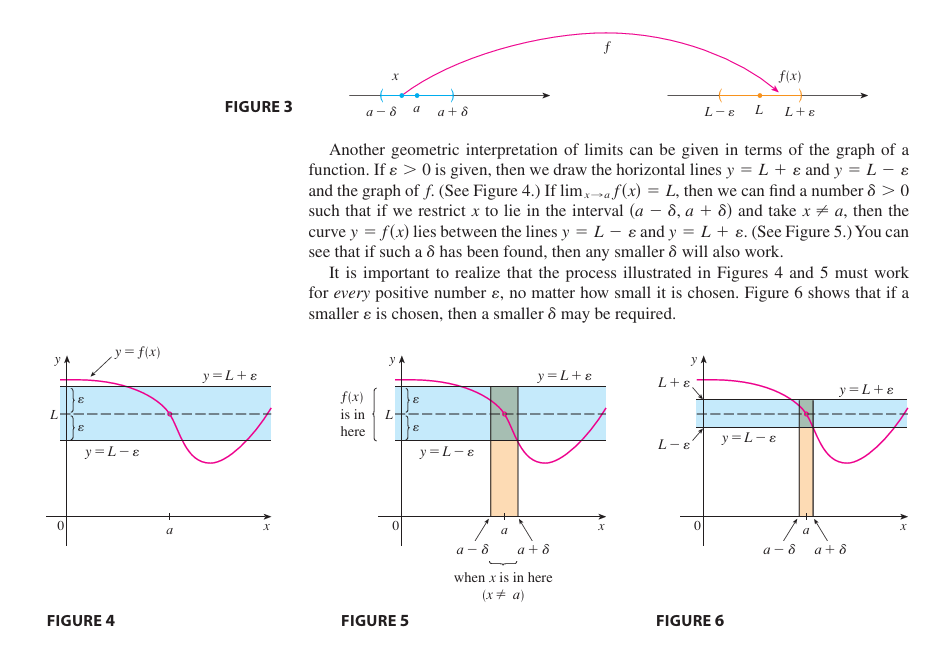
\includegraphics[width=\textwidth]{assets/calculus.png}
        \end{column}
        \begin{column}{0.3\textwidth} % 中间图片
            \centering
            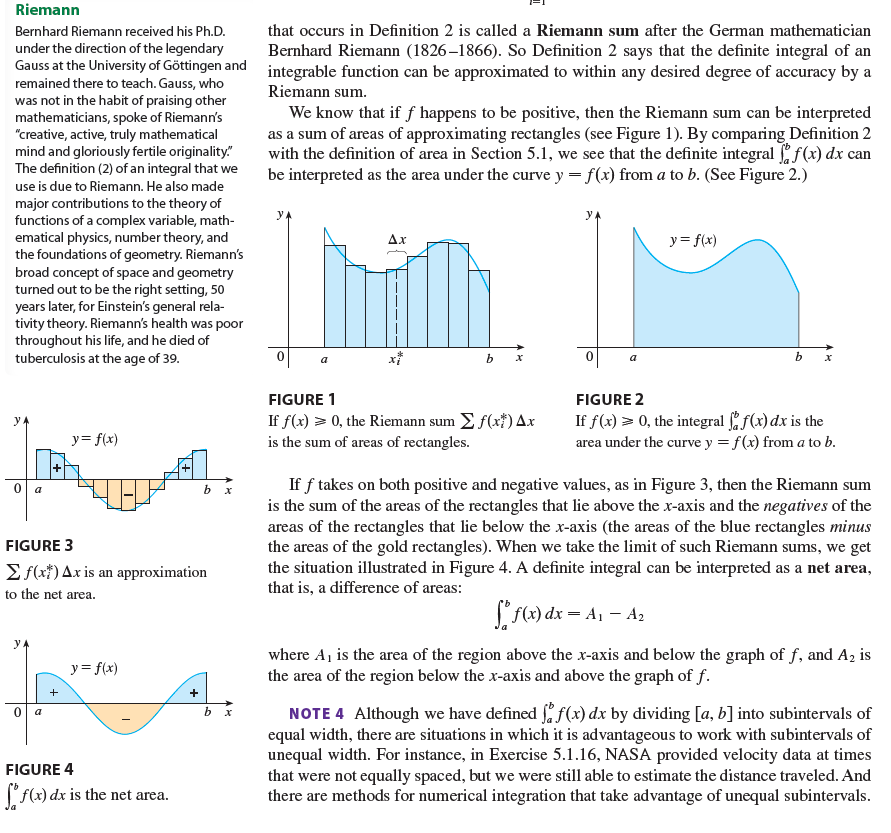
\includegraphics[width=\textwidth]{assets/calculus2.png}
        \end{column}
        \begin{column}{0.3\textwidth} % 右侧图片
            \centering
            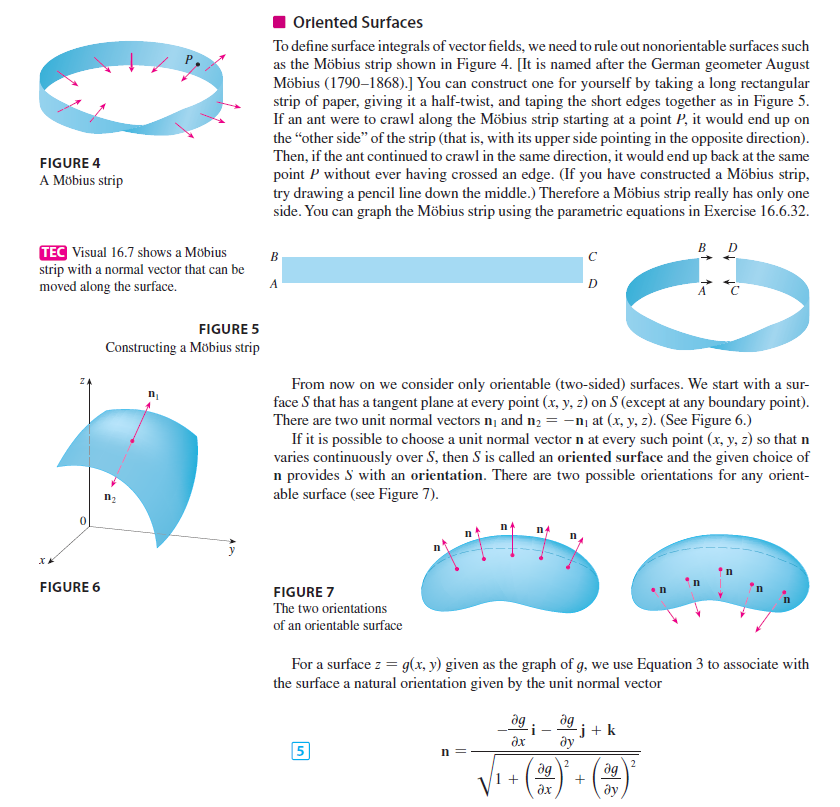
\includegraphics[width=\textwidth]{assets/calculus3.png}
        \end{column}
    \end{columns}
    
    \vspace{0.5cm} % 增加一点垂直空间,让图片不那么贴近页边
    \begin{center}
        \Large \textit{好的教材,把数学从“代码”模式,渲染成了“可视化”模式。}
    \end{center}
\end{frame}


\begin{frame}{线性代数:AI时代的“通用语言”}
\framesubtitle{世界本没有无解的问题,只有没被发现的答案}
    \begin{columns}[T]
        \begin{column}{0.5\textwidth}
            \vspace{1cm}
            \huge 你还在从\alert{行列式}开始学吗?
            
            \vfill

            \begin{flushright}
                \large
                你学的究竟是\alert{线性代数},\\
                还是矩阵行列式\alert{计算}?
            \end{flushright}

            \vfill
            
            \huge 为什么只会\alert{做题}却不懂\alert{原理}?

            \vfill
            
            % 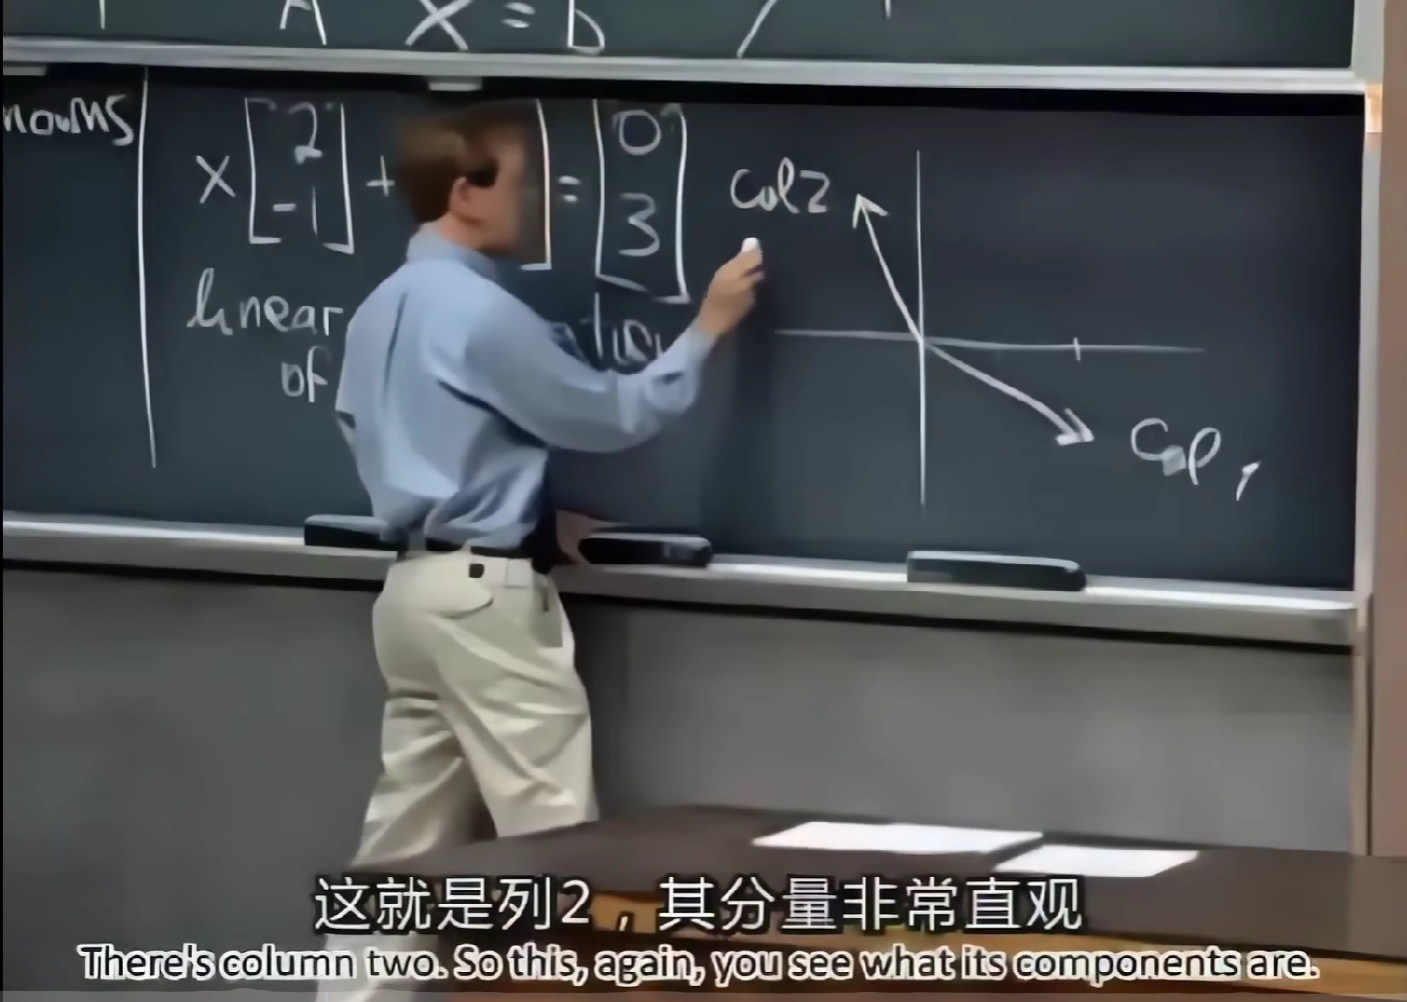
\includegraphics[width=0.6\linewidth]{assets/吉尔伯特.png}

        \end{column}
        
        \begin{column}{0.5\textwidth}
            \begin{center}
                \Large \textbf{换一种“打开方式”}
            \end{center}
            \vspace{0.3cm}
            MIT的“网红”教授 Gilbert Strang,将为你揭示线性代数的真正面貌:
            
            \begin{itemize}
                \item \textbf{神级公开课:\hrefcol{https://ocw.mit.edu/courses/18-06sc-linear-algebra-fall-2011/pages/syllabus/}{MIT 18.06}} \\
                \small 全球最受欢迎的线代课程,没有之一。老爷子用几何的直觉,带你俯瞰整个学科的脉络。
                \item \textbf{3Blue1Brown - 线性代数的本质}
                \item \textbf{配套教科书:《线性代数导论》} \\
                \small (Introduction to Linear Algebra) \\
            \end{itemize}

        \end{column}
    \end{columns}
\end{frame}

\begin{frame}
    % 致敬页不需要标题,让画面和文字自己说话
    \begin{columns}[T]
        \begin{column}{0.5\textwidth}
            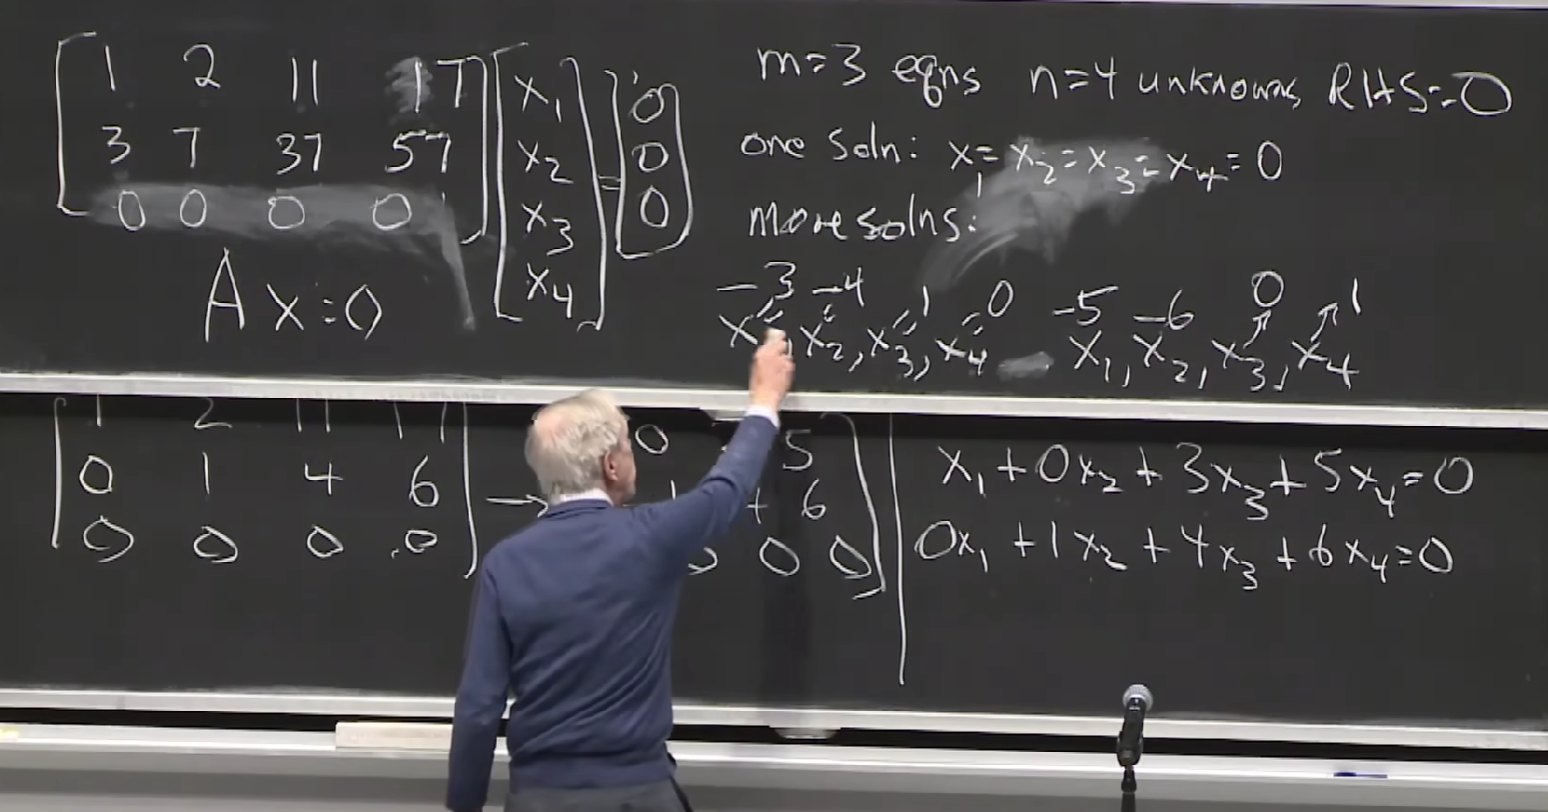
\includegraphics[width=\textwidth]{assets/linear.png}
        \end{column}
        
        \begin{column}{0.5\textwidth}
            \vspace{1cm}
            \large
            直到88岁,他依然站在讲台前。 \\
            \vspace{0.5cm}
            \Large
            甚至,连握着粉笔的手,都在微微颤抖。
            
            \vfill % 增加留白,让文字呼吸
            
            \normalsize
            几十年来,斯特朗教授为MIT,乃至全世界的学生,贡献了无数高质量的课程。
            
            \vfill

            \large
            他的退休,是一个传奇的落幕。

        \end{column}
    \end{columns}
    
    \begin{textblock*}{0.9\textwidth}(0.05\paperwidth, 0.85\paperheight)
        \begin{center}
            \textit{To Gilbert Strang,With Gratitude and Respect.}
        \end{center}
    \end{textblock*}
\end{frame}


\begin{frame}{概率论:量化“不确定性”的科学}
\framesubtitle{你说我们在一起的概率为0,但我坚信它不一定不发生}
    \begin{center}
        \large\textit{爱因斯坦曾说“上帝不掷骰子”,但在AI的世界里,\alert{万物皆由概率驱动}。}
    \end{center}
    
    \rule{\textwidth}{0.4pt}
    \vspace{0.3cm}
    
    \begin{columns}[T]
         \begin{column}{0.5\textwidth}
         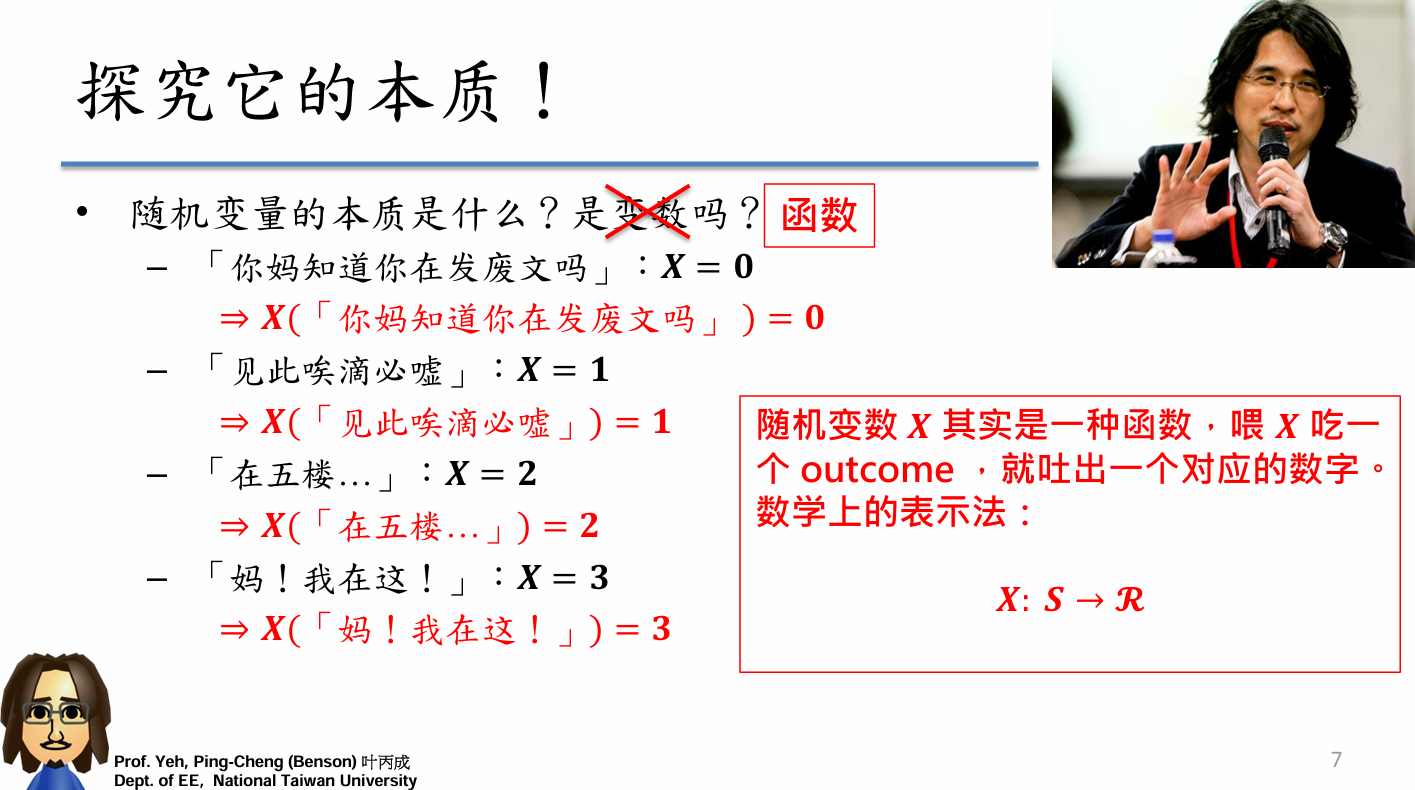
\includegraphics[width=\textwidth]{assets/prob.png}
         \end{column}
        \begin{column}{0.5\textwidth}
            % \Large\textbf{入门“神装”推荐}
            \begin{itemize}
                \item \textbf{经典教材:《概率导论》} \\
                \small (Introduction to Probability) 
                
                \item \textbf{MIT公开课} \\
                \small \hrefcol{https://ocw.mit.edu/courses/6-041sc-probabilistic-systems-analysis-and-applied-probability-fall-2013/}{MIT 6.041SC}
                
                \item \textbf{宝藏公开课 (中文)} \\
                \small 台湾国立大学 \hrefcol{https://www.coursera.org/learn/prob1/}{【頑想學概率】} \\
                \small B站/Coursera免费
            \end{itemize}
        \end{column}
    \end{columns}
\end{frame}


\begin{frame}{C语言:不只是一门语言}
\framesubtitle{hello world}
    \begin{columns}[T]
        \begin{column}{0.5\textwidth}
            \Large\textbf{一些你可能会有的疑问...}\\            \vspace{0.3cm}
            \begin{itemize}
                \item \textbf{AI写的比我好,为什么还要学?} \\
                \small 不理解底层和编程逻辑,你永远无法真正驾驭AI。
                
                \item \textbf{为什么第一门语言是C?} \\
                \small 足够底层,它会逼着你去直面内存、指针这些计算机最核心的概念。
                
                \item \textbf{这门课到底在学什么?} \\
                \small \alert{你学的绝不仅仅是语法},而是如何用最朴素的方式,与计算机的硬件直接对话,以及一种宝贵的\alert{“编程思维”}。
            \end{itemize}
        \end{column}
        
        \begin{column}{0.5\textwidth}
            \Large\textbf{新手上路指南}
            \vspace{0.5cm}
            
            \begin{alertblock}{避坑!不要看谭浩强!}
                请忘记那本红皮书,它的很多观念和代码风格已经严重过时。
            \end{alertblock}
            
            \begin{alertblock}{强力推荐:《C Primer Plus》}
            \end{alertblock}

            IDE我应该如何选择?

        \end{column}
    \end{columns}

\end{frame}

\begin{frame}{开发环境}
\framesubtitle{hello world}
    % --- 主要推荐 (使用标题+分割线) ---

    \begin{columns}[T]
        \begin{column}{0.7\textwidth}
            \huge WSL + VS Code \\
            
            \begin{itemize}
                \item \small \textbf{为什么是Linux环境(WSL)?} \\
                \small 直面\alert{编译、链接、执行}的全过程,深刻理解程序是如何“跑”起来的。
                \item \textbf{为什么是VS Code?} \\
                \small 插件生态丰富,与WSL无缝衔接,一个字:爽!!!!
            \end{itemize}
        \end{column}
        \begin{column}{0.3\textwidth}
            \begin{center}
                \vspace{1cm} % 调整垂直间距
                \hrefcol{https://code.visualstudio.com/docs/cpp/config-wsl}{\beamergotobutton{官方配置教程}}
            \end{center}
        \end{column}
    \end{columns}
    
    \vspace{0.3cm} % 增加区块间的距离

    % --- 次要推荐 ---
    \begin{columns}[T]
        \begin{column}{0.5\textwidth}
            \large\textbf{备选方案}
            % \vspace{0.2cm}
            \begin{itemize}
                \item \textbf{Windows + VS Code} \\
                \item \textbf{CLion} 或 \textbf{Visual Studio (VS)} \\
                \small \alert{Tips: JetBrains和微软都有免费学生认证!}
            \end{itemize}
        \end{column}
        \begin{column}{0.5\textwidth}
            \large\textbf{特殊用途:应试/竞赛} \\
                
                \begin{itemize}
                    \item \textbf{Dev-C++} 或 \textbf{在线OJ平台}
                \end{itemize}
        \end{column}
    \end{columns}
\end{frame}



\begin{frame}{算法和数据结构}
\framesubtitle{CS必学科目之一}
    \begin{columns}[T]
        \begin{column}{0.4\textwidth}
            \begin{figure}
                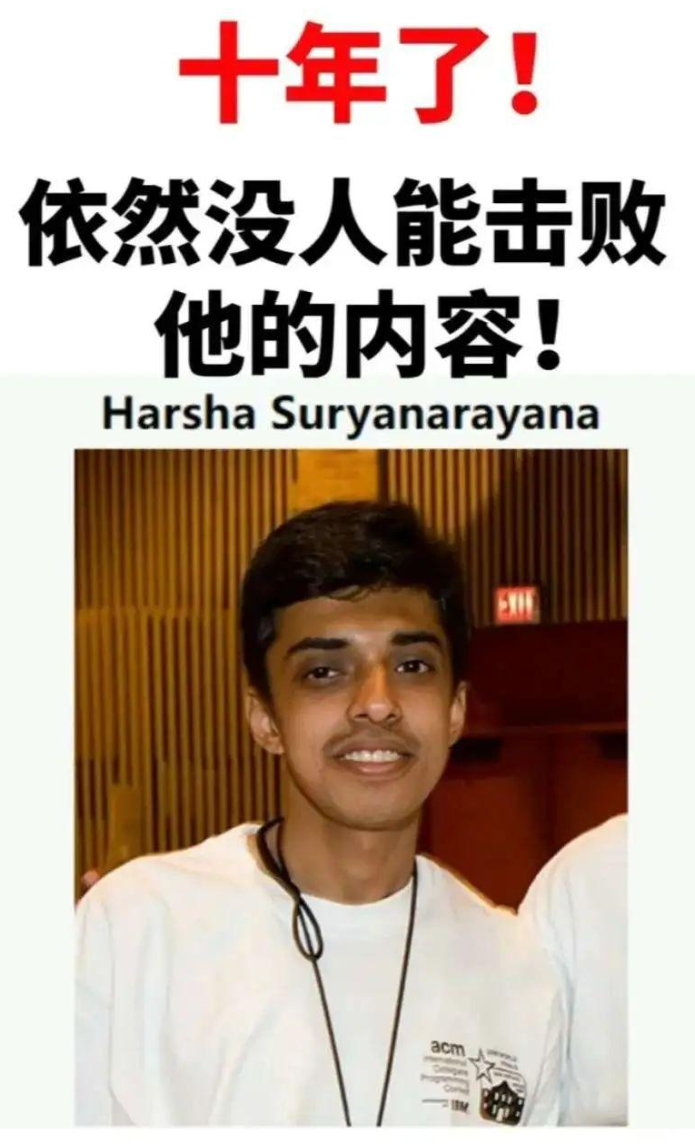
\includegraphics[width=0.7\textwidth]{assets/harsha.png}
                \caption{Harsha Suryanarayana}
            \end{figure}
        \end{column}
        
        \begin{column}{0.6\textwidth}
            \begin{itemize}
                \item \textbf{他是谁?} \\
                \small 一位来自印度的顶尖程序员,他用无可比拟的图文动画,将数据结构和指针的底层原理讲解得如诗一般清晰。
                
                \item  \textbf{他的课程}
                \begin{itemize}
                    \item \hrefcol{https://www.bilibili.com/video/BV1Fv4y1f7T1}{\small 【强烈推荐】深入浅出数据结构}
                    \item \hrefcol{https://www.bilibili.com/video/BV1iUypYyE7r/}{\small 【指针强化】4小时彻底掌握C指针}
                    
                \end{itemize}
                    \begin{alertblock}{一个令人惋惜的故事}
                        天才程序员Harsha于2014年因车祸不幸离世,年仅32岁。\\
                        但他创造的这些课程,已成为全世界无数学生的宝贵财富。\\
                        \vspace{0.3cm}
                    \end{alertblock}
            \end{itemize}
        \end{column}
    \end{columns}
\end{frame}

\begin{frame}{算法与数据结构}
    \framesubtitle{理论与实践,缺一不可}
    
    \begin{columns}[T]
        \begin{column}{0.5\textwidth}
            \Large\textbf{理论}
            \vspace{0.3cm}
            
            \begin{itemize}
                \item \textbf{《算法导论》(CLRS)$\star \star \star$}
                % \vspace{0.5cm} % 增加书籍之间的间距
                \item \textbf{《大话数据结构》$\star \star \star \star$}
                \item \textbf{B站UP蓝不过海}
                \item 一些C++语法基础
            \end{itemize}
        \end{column}
        
        \begin{column}{0.5\textwidth}
            \Large\textbf{实践}
            \vspace{0.3cm}
            
            \begin{itemize}
                \item  \textbf{LeetCode (力扣)} \\
                \item \textbf{AcWing} \\
                \item  \textbf{洛谷} \\
                \item \textbf{杭电OJ} \\
            \end{itemize}
        \end{column}
    \end{columns}

    \begin{alertblock}{忠告}
        “看懂”和“会写”之间,隔着一万行代码的距离
    \end{alertblock}
\end{frame}


\section{大二规划}
\begin{frame}{深入计算机的灵魂}
    \framesubtitle{一切,都从这本书开始...}
    
    \begin{columns}[T]
        \begin{column}{0.5\textwidth}
             \hrefcol{https://www.cs.cmu.edu/~213/}{\huge \textbf{CSAPP}}
            % --- 修改在这里 ---
            \large \textit{Computer Systems: \\ A Programmer's Perspective}

            \begin{center}
                \Large \textbf{一本打通你CS“任督二脉”的神书}
            \end{center}
            \begin{itemize}
                    \small \item 程序在内存中长什么样?
                    \item 计算机架构是什么样子的?
                    \item C代码如何变成机器指令?
                    \item CPU是如何“欺骗”你它有无限内存的?
            \end{itemize}
            
        \end{column}
        
        \begin{column}{0.5\textwidth}
            \begin{figure}
                \centering
                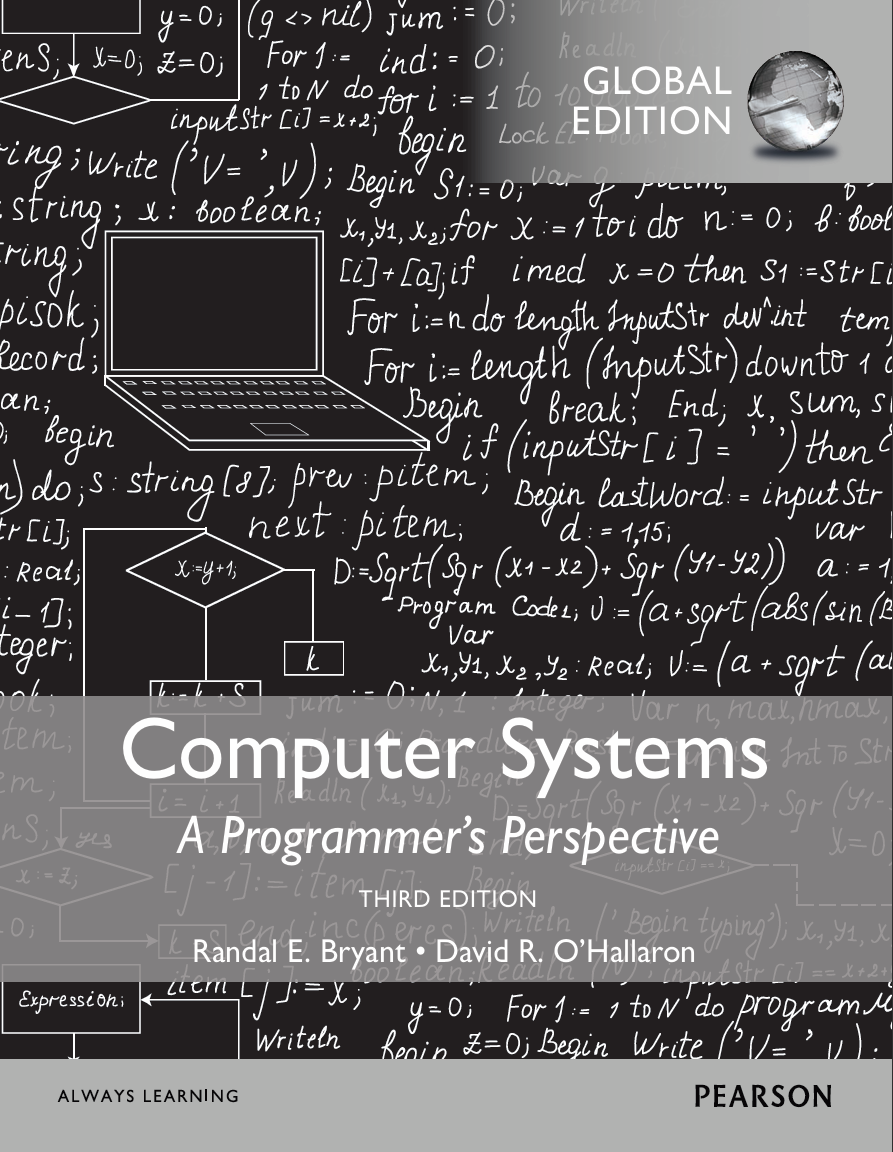
\includegraphics[width=0.7\linewidth]{assets/csapp.png}
                \caption{计算机系统的“圣经”}
            \end{figure}
        \end{column}
    \end{columns}
\end{frame}

\begin{frame}{Java \& Python}

    \begin{columns}[T]
        \begin{column}{0.5\textwidth}
            \begin{center}
                \huge Java
                \vspace{0.3cm}
                
                \large\textbf{学习目的:彻底搞懂“面向对象”}
            \end{center}
            \begin{itemize}
                \item  \textbf{思维转变:} \\
                不再是C语言那样的数据和函数分离。去构建一个个独立的\alert{“对象”(Object)}。
                
                \item 封装、继承、多态、类 、 实例
            \end{itemize}
        \end{column}
        
        \begin{column}{0.5\textwidth}
            \begin{center}
                \huge Python
                \vspace{0.3cm}
                
                \large\textbf{学习目的:把它变成你的“瑞士军刀”}
            \end{center}
            \begin{itemize}
                \item \textbf{思维转变:} \\
                第三方库。你要学会“拿来就用”,快速解决问题。

                \item 写个爬虫,抓取数据
                    \item 用Pandas/Numpy,分析数据
                    \item 为未来的\alert{机器学习}打下坚实基础、
            \end{itemize}
        \end{column}
    \end{columns}

\end{frame}

\begin{frame}{计算机组成}
    \begin{center}
        \huge CSAPP
        \vspace{0.5cm}
        
        \Large\textit{已为你铺平了90\%的道路...}
    \end{center}

    \vfill % 增加垂直间距,将内容推向两端
    \rule{\textwidth}{0.4pt}
    \vspace{0.1cm}
    

    \begin{columns}[T]
        \begin{column}{0.5\textwidth}
            \begin{center}
                \textbf{《计算机组成与设计:}  \textbf{软硬件接口》}\\
                \textbf{《计算机组成与体系结构:性能设计》}
            \end{center}
        \end{column}
        \begin{column}{0.5\textwidth}
            \begin{center}
                \textbf{《计算机体系结构:}  \textbf{量化研究方法》}
            \end{center}
        \end{column}
    \end{columns}
\end{frame}

\begin{frame}{操作系统}
    \begin{center}
        \huge \hrefcol{https://jyywiki.cn/OS/2022/index.html}{操作系统 (南京大学 - 蒋炎岩)}
        \vspace{0.5cm}
        
        \large\textit{一门“活”的、与时俱进的操作系统课}
    \end{center}

    \vfill
    \rule{\textwidth}{0.4pt}
    \vspace{0.3cm}
    

    \begin{columns}[T]
        \begin{column}{0.33\textwidth}
            \centering
            \vspace{0.5cm}
            \textbf{《操作系统导论》} \\ \small(OSTEP)
        \end{column}
        \begin{column}{0.33\textwidth}
            \centering
            \vspace{0.5cm}
            \textbf{《操作系统精髓与设计原理》}
        \end{column}
        \begin{column}{0.33\textwidth}
            \centering
            \vspace{0.5cm}
            \textbf{《操作系统概念》} \\ \small(恐龙书)
        \end{column}
    \end{columns}
\end{frame}

\begin{frame}{计算机网络}
    \begin{center}
        \Large B站两大“镇站之宝”
        \vspace{0.5cm}
        
        \huge \textbf{湖科大 - 计算机网络}
        \vspace{0.3cm}
        \huge \textbf{中科大 - 计算机网络}
    \end{center}
    
    \vfill
    \rule{\textwidth}{0.4pt}
    \vspace{0.3cm}

    \begin{columns}[T]
        \begin{column}{0.5\textwidth}
            \begin{center}
                \textbf{《计算机网络:} \\ \textbf{自顶向下方法》} \\ \small \alert{(首推)}
            \end{center}
        \end{column}
        \begin{column}{0.5\textwidth}
            \begin{center}
                \textbf{《计算机网络》} \\ \small (谢希仁 / Tanenbaum)
            \end{center}
        \end{column}
    \end{columns}
\end{frame}

\begin{frame}{数据库与分布式}
    \begin{center}
        \huge \hrefcol{https://15445.courses.cs.cmu.edu/fall2022/}{\textbf{CMU 15-445: Database Systems}}
        \large \textit{最好的数据库入门课程,没有之一}
        \large 配套书籍:《数据库系统概念》
    \end{center}
    
    \vfill
    \rule{0.8\textwidth}{0.4pt}
    \vfill

    \begin{center}
        \huge \hrefcol{https://pdos.csail.mit.edu/6.824/}{\textbf{MIT 6.824: Distributed Systems}}
        \large \textit{传说中的“神课”,Lab极具挑战性}
        \large 配套书籍:《设计数据密集型应用》(DDIA)
    \end{center}
\end{frame}

\begin{frame}
    \vfill % 增加一个弹性的垂直空白,将内容推向页面中心
    \begin{center}
        \Huge
        大二阶段
        
        \vspace{0.5cm} % 调整行间距
        
        \huge
        需要入门
        
        \vspace{0.5cm} % 调整行间距
        
        \LARGE
        \alert{至少一到两种}
        
        \vspace{0.5cm} % 调整行间距
        
        \huge
        以下的技术路线
    \end{center}
    \vfill
\end{frame}

\section{大三规划}

\begin{frame}{以项目驱动,“从战中学”}
    \framesubtitle{忘掉“学完再做”,拥抱“边做边学”}
    
    \begin{columns}[T]
        \begin{column}{0.5\textwidth}
            \Large\textbf{思维转变:项目驱动}
            \begin{itemize}
                \item  不再是“我学了Java,所以只能做个Java项目”。
                \item  而是“我想做一个电商网站,所以我需要带着 \alert{Spring Boot} 和 \alert{Vue}”。
                \item  AI时代\alert{语言语法不再是障碍!} 
                \item 跟着视频码字,第一遍盲从,第二遍理解,第三遍复刻。
            \end{itemize}

        \end{column}
        
        \begin{column}{0.5\textwidth}
            \Large\textbf{“练兵场”推荐}
            \begin{center}
                \huge YouTube
            \end{center}
            \begin{itemize}
                \item \small 例如搜索“Build a [XXX] with [MERN Stack]”,有无数手把手的顶级项目教程。
            \end{itemize}
            
            
            \begin{center}
                \huge 官方文档 (Official Docs)
            \end{center}
            \begin{itemize}
                \item \small 永远的第一手信息源。90\%的答案都在官方入门教程里。
            \end{itemize}
        \end{column}
    \end{columns}
    
\end{frame}

\begin{frame}{项目路线 (一):全栈Web开发$\star \star \star \star \star$}
    \framesubtitle{构建现代互联网应用,实习/求职的“王道征途”}

    \begin{columns}[T]
        \begin{column}{0.5\textwidth}
            \Large \textbf{后端技术栈 (Backend)}
            \begin{itemize}
                \item Java (\alert{Spring Boot})
                \item Python (Django / Flask / FastAPI)
                \item Go (Gin)
                \item Node.js (Express / Koa)
            \end{itemize}
        \end{column}
        \begin{column}{0.5\textwidth}
            \Large \textbf{前端框架 (Frontend)}
            \begin{itemize}
                \item \alert{Vue.js}
                \item React
            \end{itemize}
        \end{column}
    \end{columns}
    
    \vfill
    \rule{\textwidth}{0.4pt}
    \vfill
    
    \begin{columns}[T]
        \begin{column}{0.5\textwidth}
            \Large \textbf{数据层 (Data)}
            \begin{itemize}
                \item \textbf{数据库:} MySQL, MongoDB
                \item \textbf{缓存:} Redis
            \end{itemize}
        \end{column}
        \begin{column}{0.5\textwidth}
            \Large \textbf{设计与原型 (UI/UX)}
            \begin{itemize}
                \item \textbf{Figma}: \small 产品/设计/开发协作必备
            \end{itemize}
        \end{column}
    \end{columns}
    
\end{frame}

\begin{frame}{项目路线 (二):客户端开发$\star \star \star$}
    \framesubtitle{打造触手可及的桌面与移动应用}

    \begin{columns}[T]
        \begin{column}{0.5\textwidth}
            \begin{center}
                \huge 移动端 App
            \end{center}
            \begin{itemize}
                \item \textbf{跨平台 (首推):} \\ Flutter, React Native
                \item \textbf{小程序} \\ Uniapp
                \item \textbf{原生开发:} \\ Android (Kotlin), 鸿蒙开发
            \end{itemize}
        \end{column}
        \begin{column}{0.5\textwidth}
            \begin{center}
                \huge 桌面端 GUI
            \end{center}
            \begin{itemize}
                \item \textbf{原生体验:} \\ Qt (C++), WPF (C\#)
                \item \textbf{Web壳子:} \\ Electron, Tauri
            \end{itemize}
        \end{column}
    \end{columns}
    
\end{frame}

\begin{frame}{项目路线 (三):人工智能$\star \star \star \star \star$}
    \framesubtitle{开启未来的钥匙,时代的终极浪潮}
    
    \begin{columns}[T]
        % --- 左侧:基础与入门 ---
        \begin{column}{0.5\textwidth}
            \begin{center}
                \large\textbf{打好数学与工具基础}
                \rule{0.8\linewidth}{0.4pt}
            \end{center}
            \begin{itemize}
                \item 三大神器:Numpy, Pandas, Matplotlib
            \end{itemize}

            \vfill

            \begin{center}
                \large\textbf{跟随大师系统入门}
                \rule{0.8\linewidth}{0.4pt}
            \end{center}
            \begin{itemize}
                \item 吴恩达 \hrefcol{https://www.coursera.org/learn/machine-learning}{机器学习}
                \item 吴恩达 \hrefcol{https://www.coursera.org/specializations/deep-learning}{深度学习} 专项
            \end{itemize}
        \end{column}

        % --- 右侧:框架与实战 ---
        \begin{column}{0.5\textwidth}
            \begin{center}
                \large\textbf{掌握核心框架}
                \rule{0.8\linewidth}{0.4pt}
            \end{center}
            \begin{itemize}
                \item PyTorch \textit{(学术界首选)}
                \item TensorFlow \textit{(工业界常用)}
            \end{itemize}

            \vfill

            \begin{center}
                \large\textbf{投身实战与前沿}
                \rule{0.8\linewidth}{0.4pt}
            \end{center}
            \begin{itemize}
                \item \alert{Kaggle} 项目实战
                \item 经典 \alert{Paper} 精读
                \item 前沿方向:大语言模型(LLM), Agent
            \end{itemize}
        \end{column}
    \end{columns}
\end{frame}


\begin{frame}{项目路线 (四):游戏开发$\star \star$}
    \framesubtitle{从“玩家”到“造物主”,创造属于你的世界}
    
    \begin{columns}[T]
        \begin{column}{0.33\textwidth}
            \centering
            \huge Unity
            \small (C\#)
            \vfill
            行业标杆,生态成熟,移动/独立游戏首选。
        \end{column}
        \begin{column}{0.33\textwidth}
            \centering
            \huge Godot
            \small (GDScript/C\#)
            \vfill
            开源免费,轻量易上手,社区驱动的潜力股。
        \end{column}
        \begin{column}{0.33\textwidth}
            \centering
            \huge UE
            \small (C++/蓝图)
            \vfill
            画质巅峰,3A大作之选,对初学者有门槛。
        \end{column}
    \end{columns}

    \vfill
    \begin{alertblock}{入门建议}
        从复刻一个经典2D游戏(如俄罗斯方块、贪吃蛇)开始你的“创世之旅”。
    \end{alertblock}
\end{frame}

\begin{frame}{项目路线 (五):硬件 / 嵌入式$\star \star \star$}
    \framesubtitle{让代码感知并控制物理世界}
    
    \begin{columns}[T]
        \begin{column}{0.5\textwidth}
            \begin{center}
                \huge Arduino
                \vspace{0.3cm}
                
                \large\textbf{“电子积木”,极易上手}
            \end{center}
            \begin{itemize}
                \item \textbf{控制语言:} C/C++

            \end{itemize}
        \end{column}
        
        \begin{column}{0.5\textwidth}
            \begin{center}
                \huge Raspberry Pi
                \large (树莓派)
                \vspace{0.3cm}
                
                \large\textbf{“口袋电脑”,性能更强}
            \end{center}
            \begin{itemize}
                \item \textbf{控制语言:} Python
            \end{itemize}
        \end{column}
    \end{columns}
    

\end{frame}

\begin{frame}{项目路线 (六):大数据技术 $\star \star \star \star$}
    \vfill % 垂直居中
    
    \begin{center}
        \Huge Hadoop \quad \quad \alert{\Huge Spark}
    \end{center}
    
    \vfill
    
    \begin{center}
        \huge Kafka \quad \quad \alert{\Huge Flink}
    \end{center}
    
    \vfill
    
    \begin{center}
        \huge Hive \quad \quad \huge HBase
    \end{center}
    
    \vfill
\end{frame}

\section{大四规划}

\begin{frame}{大四:转折点}
    \framesubtitle{}
    \begin{center}
        \Huge 無
    \end{center}

\end{frame}

\begin{frame}{毕业以后}
    \uncover{
    \begin{center}
        \vspace{0.2cm}
        
        \large
        \textit{毕业证只是你进入这个行业的一张门票,} \\
        \textit{而不是终身饭票。} \\
        \textit{CS是一个需要你终身“刷新”自己的行业。}
    \end{center}
    }
    
    \vfill
    
    \uncover {
    \begin{center}
        \vspace{0.2cm}
        
        \large
        \textit{考上名校的研究生、找到大厂的好工作...} \\
        \textit{请记住,这既非你人生幸福的\alert{充分条件},} \\
        \textit{也非你自我价值的\alert{必要条件}。}
    \end{center}
    }
    
    \vfill
    
    \uncover {
    \begin{center}
        \vspace{0.2cm}

        \large
        \textit{不要盲目追逐热点,去找到那个让你寝食难安的方向。} \\
        \textit{那份热爱,才是你抵御一切风浪与倦怠的,} \\
        \textit{最终极的动力。}
    \end{center}
    }
\end{frame}

% \begin{frame}{Beamer for SINTEF slides}
% \begin{itemize}
% \item We assume you can use \LaTeX; if you cannot,
% \hrefcol{http://en.wikibooks.org/wiki/LaTeX/}{you can learn it here}
% \item Beamer is one of the most popular and powerful document
% classes for presentations in \LaTeX
% \item Beamer has also a detailed
% \hrefcol{http://www.ctan.org/tex-archive/macros/latex/contrib/beamer/doc/beameruserguide.pdf}{user
%  manual}
% \item Here we will present only the most basic features to get you up to speed
% \end{itemize}
% \end{frame}

% \begin{frame}{Beamer vs. PowerPoint}
% Compared to PowerPoint, using \LaTeX\ is better because:
% \begin{itemize}
% \item It is not What-You-See-Is-What-You-Get, but
% What-You-\emph{Mean}-Is-What-You-Get:\\
% you write the content, the computer does the typesetting
% \item Produces a \texttt{pdf}: no problems with fonts, formulas,
%       program versions
% \item Easier to keep consistent style, fonts, highlighting, etc.
% \item Math typesetting in \TeX\ is the best:
% \begin{equation*}
% \mathrm{i}\,\hslash\frac{\partial}{\partial t} \Psi(\mathbf{r},t) =
% -\frac{\hslash^2}{2\,m}\nabla^2\Psi(\mathbf{r},t)
% + V(\mathbf{r})\Psi(\mathbf{r},t)
% \end{equation*}

% \end{itemize}
% \end{frame}

% \begin{frame}[fragile]{Getting Started}
% \framesubtitle{Selecting the SINTEF Theme}
% To start working with \texttt{sintefbeamer}, start a \LaTeX\ document with the
% preamble:
% \begin{block}{Minimum SINTEF Beamer Document}
% \verb|\documentclass{beamer}|\\
% \verb|\usetheme{sintef}|\\
% \verb|\begin{document}|\\
% \verb|\begin{frame}{Hello, world!}|\\
% \verb|\end{frame}|\\
% \verb|\end{document}|\\
% \end{block}
% \end{frame}

% \begin{frame}[fragile]{Title page}
% To set a typical title page, you call some commands in the preamble:
% \begin{block}{The Commands for the Title Page}
% \begin{verbatim}
% \title{Sample Title}
% \subtitle{Sample subtitle}
% \author{First Author, Second Author}
% \date{\today} % Can also be (ab)used for conference name &c.
% \end{verbatim}
% \end{block}
% You can then write out the title page with \verb|\maketitle|.

% To set a \textbf{background image} use the \verb|\titlebackground| command 
% before \verb|\maketitle|; its only argument is the name (or path) of a graphic 
% file.

% If you use the \textbf{starred version} \verb|\titlebackground*|, the image 
% will be clipped to a split view on the right side of the title slide.

% \end{frame}

% \begin{frame}[fragile]{Writing a Simple Slide}
% \framesubtitle{It's really easy!}
% \begin{itemize}[<+->]
% \item A typical slide has bulleted lists
% \item These can be uncovered in sequence
% \end{itemize}
% \begin{block}{Code for a Page with an Itemised List}<+->
% \begin{verbatim}
% \begin{frame}{Writing a Simple Slide}
%   \framesubtitle{It's really easy!}
%   \begin{itemize}[<+->]
%     \item A typical slide has bulleted lists
%     \item These can be uncovered in sequence
%   \end{itemize}\end{frame}
% \end{verbatim}
% \end{block}
% \end{frame}

% \section{Personalization}

% \footlinecolor{sintefyellow}
% \begin{frame}[fragile]{Changing Slide Style}
% \begin{itemize}
% \item You can select the white or \textit{maincolor} \textbf{slide style} \emph{in the 
% preamble} with \verb|\themecolor{white}| (default) or \verb|\themecolor{main}|
%       \begin{itemize}
%       \item You should \emph{not} change these within the document: Beamer does 
%       not like it
%       \item If you \emph{really} must, you may have to add 
%       \verb|\usebeamercolor[fg]{normal text}| in the slide
%       \end{itemize}
% \item You can change the \textbf{footline colour} with 
% \verb|\footlinecolor{color}|
%       \begin{itemize}
%       \item Place the command \emph{before} a new \verb|frame|
%       \item There are four ``official'' colors: 
%       \testcolor{maincolor},\testcolor{sintefyellow}, 
%       \testcolor{sintefgreen}, \testcolor{sintefdarkgreen}
%       \item Default is no footline; you can restore it with 
%       \verb|\footlinecolor{}|
%       \item Others may work, but no guarantees!
%       \item Should \emph{not} be used with the \verb|maincolor| theme!
%       \end{itemize}
% \end{itemize}
% \end{frame}

% \begin{frame}[fragile]{Blocks}
% \begin{columns}
% \begin{column}{0.3\textwidth}
% \begin{block}{Standard Blocks}
% These have a color coordinated with the footline (and grey in the blue theme)
% \begin{verbatim}
% \begin{block}{title}
% content...
% \end{block}
% \end{verbatim}
% \end{block}
% \end{column}
% \begin{column}{0.7\textwidth}
% \begin{colorblock}[black]{sinteflightgreen}{Colour Blocks}
% Similar to the ones on the left, but you pick the colour. Text will be white by 
% default, but you may set it with an optional argument.
% \small
% \begin{verbatim}
% \begin{colorblock}[black]{sinteflightgreen}{title}
% content...
% \end{colorblock}
% \end{verbatim}
% \end{colorblock}
% The ``official'' colours of colour blocks are: \testcolor{sinteflilla}, 
% \testcolor{maincolor}, \testcolor{sintefdarkgreen}, and 
% \testcolor{sintefyellow}.
% \end{column}
% \end{columns}
% \end{frame}

% \footlinecolor{}
% \begin{frame}[fragile]{Using Colours}
% \begin{itemize}[<alert@2>]
%   \item You can use colours with the
%         \verb|\textcolor{<color name>}{text}| command
%   \item The colours are defined in the \texttt{sintefcolor} package:
%   \begin{itemize}
%   \item Primary colours: \testcolor{maincolor} and its sidekick 
%   \testcolor{sintefgrey}
%   \item Three shades of green: \testcolor{sinteflightgreen}, 
%   \testcolor{sintefgreen}, \testcolor{sintefdarkgreen}
%   \item Additional colours: \testcolor{sintefyellow}, \testcolor{sintefpurple}, 
%         \testcolor{sinteflilla}, testcolor{nuaablue}
%         \begin{itemize}
%         \item These may be shaded---see the \verb|sintefcolor| documentation or 
%         the \hrefcol{https://sintef.sharepoint.com/sites/stottetjenester/%
%         kommunikasjon/grafisk-profil-new/Sider/default.aspx}{SINTEF profile 
%         manual}
%         \end{itemize}
%   \end{itemize}
%   \item Do \emph{not} abuse colours: \verb|\emph{}| is usually enough
%   \item Use \verb|\alert{}| to bring the \alert<2->{focus} somewhere
%   \item<2- | alert@2> If you highlight too much, you don't highlight at all!
% \end{itemize}
% \end{frame}

% \begin{frame}[fragile]{Adding images}
% \begin{columns}
% \begin{column}{0.7\textwidth}
% Adding images works like in normal \LaTeX:
% \begin{block}{Code for Adding Images}
% \begin{verbatim}
% \usepackage{graphicx}
% % ...
% \includegraphics[width=\textwidth]
% {assets/sdu_logo}
% \end{verbatim}
% \end{block}
% \end{column}
% \begin{column}{0.3\textwidth}
% \includegraphics[width=\textwidth]
% {assets/sdu_logo}
% \end{column}
% \end{columns}
% \end{frame}

% \begin{frame}[fragile]{Splitting in Columns}
% Splitting the page is easy and common;
% typically, one side has a picture and the other text:
% \begin{columns}
% \begin{column}{0.6\textwidth}
% This is the first column
% \end{column}
% \begin{column}{0.3\textwidth}
% And this the second
% \end{column}
% \end{columns}
% \begin{block}{Column Code}
% \begin{verbatim}
% \begin{columns}
%     \begin{column}{0.6\textwidth}
%         This is the first column
%     \end{column}
%     \begin{column}{0.3\textwidth}
%         And this the second
%     \end{column}
%     % There could be more!
% \end{columns}
% \end{verbatim}
% \end{block}
% \end{frame}

% \begin{chapter}[assets/sdubackground_negative]{}{Special Slides}
% \begin{itemize}
% \item Chapter slides
% \item Side-picture slides
% \end{itemize}
% \end{chapter}

% \footlinecolor{sintefpurple}
% \begin{frame}[fragile]{Chapter slides}
% \begin{itemize}
% \item Similar to \verb|frame|s, but with a few more options
% \item Opened with \verb|\begin{chapter}[<image>]{<color>}{<title>}|
% \item Image is optional, colour and title are mandatory
% \item There are seven ``official'' colours: \testcolor{maincolor}, 
% \testcolor{sintefdarkgreen}, \testcolor{sintefgreen}, 
% \testcolor{sinteflightgreen}, \testcolor{sintefpurple}, \testcolor{sintefyellow}, 
% \testcolor{sinteflilla}, \testcolor{nuaablue}, \testcolor{nuaalightblue}.
%       \begin{itemize}
%       \item Strangely enough, these are \emph{more} than the official colours 
%       for the footline.
%       \item It may still be a nice touch to change the footline of following 
%       slides to the same color of a chapter slide. Your choice.
%       \end{itemize}
% \item Otherwise, \verb|chapter| behaves just like \verb|frame|.
% \end{itemize}
% \end{frame}

% \begin{sidepic}{assets/sduview}{Side-Picture Slides}
% \begin{itemize}
% \item Opened with \texttt{$\backslash$begin\{sidepic\}\{<image>\}\{<title>\}}
% \item Otherwise, \texttt{sidepic} works just like \texttt{frame}
% \end{itemize}
% \end{sidepic}

% \footlinecolor{maincolor}
% \begin{frame}
% \frametitle{Fonts}
% \begin{itemize}
% \item The paramount task of fonts is being readable
% \item There are good ones...
%   \begin{itemize}
%   \item {\textrm{Use serif fonts only with high-definition projectors}}
%   \item {\textsf{Use sans-serif fonts otherwise (or if you simply prefer 
% them)}}
%   \end{itemize}
% \item ... and not so good ones:
%   \begin{itemize}
%   \item {\texttt{Never use monospace for normal text}}
%   \item {\frakfamily Gothic, calligraphic or weird fonts: should always: be
%   avoided}
% \end{itemize}
% \end{itemize}
% \end{frame}

% \begin{frame}[fragile]{Look}
% \begin{itemize}
% \item To insert a final slide with the title and final thanks, use \verb|\backmatter|.
%       \begin{itemize}
%       \item The title also appears in footlines along with the author name, you can change this text with \verb|\footlinepayoff|
%       \item You can remove the title from the final slide with \verb|\backmatter[notitle]|
%       \end{itemize}
% \item The aspect ratio defaults to 16:9, and you should not change it to 4:3
%       for old projectors as it is inherently impossible to perfectly convert a 
%       16:9 presentation to 4:3 one; spacings \emph{will} break
%       \begin{itemize}
%       \item The \texttt{aspectratio} argument to the \texttt{beamer} class is
%             overridden by the SINTEF theme
%       \item If you \emph{really} know what you are doing, check the package
%             code and look for the \texttt{geometry} class.
%       \end{itemize}
% \end{itemize}
% \end{frame}


% \begin{frame}
% \frametitle{Good Luck!}
% \begin{itemize}
% \item Enough for an introduction! You should know enough by now
% \item If you have corrections or suggestions,
% \hrefcol{mailto:2861126078@qq.com}{send them to me!}
% \end{itemize}
% \end{frame}

\backmatter
\end{document}
